\chapter{Methodology}
\label{chap:method}

In this section, the methodology of the proposed solution is explained in detail. This section is divided into sequential subsections that each describe a step in the process used to arrive at the proposed dataset, the formulation of the analytical problem to be solved, and the \acrfull{ml} related data preparation, training, and evaluation.

\section{General approach overview}

Based on the findings from the literature review conducted in \cref{sec:lit_review}, it is clear that the existing work is limited in terms of a general and global prediction solution for vessel destination ports. Thus, this thesis proposes a method that is able to predict vessels' future destination ports using a combination of positional data from the \gls{aivdm} protocol and vessel segmentation values. This is an important objective of the thesis as no related studies seem to take additional vessel information into account. The proposed solution is not restricted by specific geographical regions nor time intervals and should form a foundation of which it is possible to extend with more features, or data attributes, regarding the traveling vessels and voyages. The method of developing the proposed solution can be divided into the following steps:

\begin{enumerate}
    \item Construct voyages and trajectories using a voyage definition derived from the departure and arrival detection described in \cref{sec:vessel_transitions}.
    \item Sample, or simplify, the trajectories to make them more comparable using vessel similarity measurement methods.
    \item Calculate the \acrfull{mstd} and the similarity value for every voyage's trajectory.
    \item Collect the historical data attributes to be used for \acrfull{ml} including departure and arrival ports, vessel segmentation values, \acrshort{mstd} values, and trajectory lengths.
    \item Train a \acrshort{ml} model to predict the arrival ports of voyages using the dataset constructed.
\end{enumerate}

\section{The initial data processing}

This section describes the initial dataset used in the proposed solution which is later processed and used to train a \acrshort{ml} model for predictions. This data foundation is provided to the author by \acrfull{mo}. Moreover, for this thesis, data used in the analysis is stored in a separate, dedicated PostgreSQL database also hosted in \acrshort{mo}'s cloud computing environment.

\subsection{Positional historical AIS data}

The first step in the dataset processing is to collect a historical set of \acrshort{ais} data. In this thesis, this data provided by \acrshort{mo} contains more than 1.5 billion positional records for over 65 000 unique vessels starting from December 2019 and is continuously collected. In this thesis, circa 1.2 billion records ranging from December 2019 to March 2021 were used for the proposed solution. The historical records were copied in batches from \acrshort{mo}'s database into a separate database used in this thesis in a table called \textit{vessel positions history}. This table contains the following relevant attributes for each historical record:

\begin{itemize}
    \item id - a sequential identifier
    \item imo - the \acrshort{imo} number of the vessel that transmitted the position.
    \item mmsi - the \acrshort{mmsi} number of the vessel that transmitted the position.
    \item position - a geographical coordinate of the vessel in the \textit{Mercator} projection.
    \item timestamp - the UNIX timestamp (seconds since Unix Epoch) of when the position was transmitted by the vessel.
\end{itemize}

In the process of copying data to the dedicated database, each position's coordinate is validated by ensuring that it follows the bounds its projection, i.e., that the longitude value is between -180, and 180 degrees and the latitude is between -90, and 90 degrees. If a coordinate has invalid values, it is disregarded. Furthermore, positions that lie exactly on the north and south bounds, or exactly at coordinates \textit{(180, 90)} and \textit{(-180, -90)} are also disregarded as these positions are impossible places to navigate but are still frequently seen in the database. \cref{fig:ais_positions} in \cref{sec:ais_data} shows a visualization of an extract of 100 million records from the historical \acrshort{ais} database which shows the extent of the collected positions.

Furthermore, as also mentioned in \cref{sec:ais_data}, \acrshort{imo} numbers and \acrshort{mmsi} numbers are divided up in the positional and static \acrshort{ais} reports. Therefore, \acrshort{mmsi} numbers in positional data must be matched to \acrshort{imo} numbers in the static information (which contains both) to collect both identifiers in the historical \acrshort{ais} database. The \acrshort{imo} identifier is required to extract information such as vessel segments and sub-segments as these are initially constructed using information from static records. Positions transmitted by a \acrshort{mmsi} number that does not map to a known \acrshort{imo} number, or have invalid values for either, are disregarded. The validity of both values can be determined following the \gls{aivdm} protocol which defines how these numbers are constructed and used.

\subsection{Segments}

As described in \cref{sec:vessel_info_segments}, vessel segmentation values are additional attributes that indicate a vessel's type, dimensions, and capacity. These labels are thought to provide insight into the traveling patterns of vessels. Thus, this information is important for this thesis's proposed solution. \acrshort{mo} has vessel segmentation information for every unique vessel collected by \acrshort{ais} data. This information is collected and stored in the dedicated database in a table called \textit{vessel segments}. This table contains information per vessel and has the following relevant attributes:

\begin{itemize}
    \item imo - the \acrshort{imo} number of the vessel.
    \item segment - the vessel's segment value, e.g. \textit{dry bulk}, \textit{tanker}, \textit{chemical}, etc\ldots
    \item sub-segment - the vessel's sub-segment value, e.g., \textit{mini bulker}, \textit{handysize}, \textit{Panamax}, etc\ldots
\end{itemize}

Finally, it is worth noting that some vessels can function as two different types of vessels such as tanker vessels that also function as chemical transport vessels. These ``combo'' vessels contain multiple entries in the segmentation database table for each of the functions it serves. However, they also contain a dedicated entry where the segment value is ``combo'' which can have a specific range of sub-segments. For analysis, it is more practical to assume that every vessel only has one segment and one sub-segment, therefore, for combo vessels, only the combo segment and sub-segment are considered.

\subsection{Ports}

Next, the traveling vessel's departure and arrival port are required to predict vessels' future destinations, as destinations are defined ports. As already described in \cref{sec:shipping_ports}, \acrshort{mo} has a large number of ports available in a port database out of which around 5600 are considered relevant for the shipping industry. For this thesis, only these 5600 relevant ports are considered for the analysis, thus, these are also stored in the dedicated database in a table called ``ports''. This table contains the following relevant attributes:

\begin{itemize}
    \item locode - the port's unique identifier following the \gls{locode} protocol.
    \item position - the port's geographical coordinates specified in the Mercator projection.
    \item name - a text value for the name of the port.
\end{itemize}

\subsection{Vessel transitions}

As described in \cref{sec:vessel_transitions}, vessel transitions are historical events where a vessel's \acrshort{ais} navigational status transitions from a status indicating that it is moving to the status ``MOORED'' and vice versa. These events are mapped geographically to the closest known port within a 25-kilometer radius, thus, vessel transitions provide a historical record of port arrivals and departures. \acrshort{mo} has more information available in their transition data, however, only vessel arrival and departure data are of relevance to the proposed solution. The relevant data is stored in the dedicated database as a table called \textit{vessel transitions}. This table contains vessel identifiers, the event's mapped port, the Unix timestamp of when the event occurred, and the transition type indicating whether the vessel arrived or departed. \cref{tab:vessel_transitions_example} shows an example extract from the transitions data for a single vessel. It shows that when sorted by time, the events follow a pattern of sequential arrival and departures from different ports.

\begin{table}[htbp]
    \centering
    \begin{tabular}{p{0.7in} p{0.9in} p{1in} p{1in} p{0.65in}}
    \hline
    \bfseries{IMO} & \bfseries{MMSI} & \bfseries{Transition} & \bfseries{Timestamp} & \bfseries{Port Code} \\ \hline
        9824083 & 538008866 & ARRIVAL   & 1595383670 & KRONS \\ \hline
        9824083 & 538008866 & DEPARTURE & 1596177702 & KRONS \\ \hline
        9824083 & 538008866 & ARRIVAL   & 1599869735 & BRITQ \\ \hline
        9824083 & 538008866 & DEPARTURE & 1600002777 & BRITQ \\ \hline
        9824083 & 538008866 & ARRIVAL   & 1603942962 & CNZNG \\ \hline
        9824083 & 538008866 & DEPARTURE & 1604191770 & CNZNG \\ \hline
    \end{tabular}
\caption{Example rows for a single vessel in the vessel transitions table}
\label{tab:vessel_transitions_example}
\end{table}

\section{Vessel voyage definition}

After the initial data foundation is constructed as described in the previous section, the next step is to construct voyages and voyage trajectories based on the historical \acrshort{ais} data. As described in \cref{sec:vessel_voyage_definition}, throughout this thesis, a vessel voyage has been defined based on vessel transitions derived from \acrshort{ais} navigational statuses. This is mainly because it is thought to provide more valuable predictions for the actors in the industry. This hypothesis was confirmed by the collaborative company \acrfull{mo} but has also been corroborated by interviewing real actors in the industry as will be later discussed in \cref{chap:results}. This section describes the methods tested and used to construct voyages from the initial data foundation described up to this point in \cref{chap:method}.

\subsection{Cluster-based voyages}

\todo{Should I bother explaining work I did with clustering if I didn't use it in the final approach?}

\subsection{Transition voyages}

As vessel transitions provide a historical record per vessel of arrivals and departures based on \acrshort{ais} statuses it can be used to derive vessel voyages. Given two entries in the vessel transitions table for a single vessel, sorted by time, where the first is a departure from a port, and the second is arrival at another port, a voyage can be defined as starting at the timestamp of the first departure transition and ending at the subsequent arrival transition. For example, in \cref{tab:vessel_transitions_example}, there are six transition events for a single vessel ordered by time. Based on these events, two different voyages can be defined:

\begin{enumerate}
    \item  Vessel departed port \textit{KRONS} on the 31st of July 2020 and arrived at port \textit{BRITQ} on the 12th of September 2020.
    \item  Vessel departed port \textit{BRITQ} on the 13th of September 2020 and arrived at port \textit{CNZNG} on the 29th of October 2020.
\end{enumerate}

Using the vessel transition information, the first step is to deduce voyages based on sequential arrival and departures for vessels. After a voyage has been defined, the second step is to find the trajectory of the traveling vessel. This can be deduced from the vessel positions history table as every \acrshort{ais} positional report transmitted between the derived departure and arrival timestamps from the traveling vessel forms a geographical trajectory from the departure and arrival port.

\subsubsection{Constructing voyages}

Constructing voyages based on vessel transitions and positional records can be summarized in the following steps:

\begin{enumerate}
    \item Extract vessel transitions per vessel ordered by time.
    \item Define voyages based on subsequent departures and arrivals from the vessel transition data (\cref{lst:voyage_times}).
    \item For each voyage, extract every positional record between vessels' departure and arrival timestamps sorted by time.
    \item Validate the geographical trajectory including applying a ``noise filter'' (\cref{fig:noise_filter}).
    \item Store voyages with validated trajectories in transition voyages table.
\end{enumerate}

The first step including defining trajectories based on vessel transitions is a relatively straightforward process of looking for transitions following the pattern of departures immediately followed by arrival at a different port. The algorithm used to compute voyages based on a vessel's transition events is shown in \cref{lst:voyage_times}.

\begin{lstlisting}[
    caption={Golang code used to compute voyage times from vessel transitions. The code has been reduced slightly for readability.},
    label=lst:voyage_times,
    language=Go,
    showstringspaces=false,
]
func getVoyageTimes(transitions []VesselTransition) []Voyage {
	var voyages []Voyage
	j := 0
	for i, current := range transitions {
                // start at the first departure event
		if current.Transition != "DEPARTURE" {
			continue
                // get the subsequent transition
		j = i + 1
		if j >= len(transitions) {
			break
		}
		next := transitions[j]

                // ensure the next event is an arrival at a different port
		if next.Transition != "ARRIVAL" {
			continue
		}
		if current.PortCode == next.PortCode {
			continue
		}

		voyages = append(voyages, Voyage{
			IMO:                current.IMO,
			MMSI:               current.MMSI,
			DeparturePort:      current.PortCode,
			DepartureTimestamp: current.Timestamp,
			ArrivalPort:        next.PortCode,
			ArrivalTimestamp:   next.Timestamp,
		})
	}
	return voyages
}
\end{lstlisting}

Next, the voyage times computed are used to construct geographical trajectories. This process is, in essence, a simple matter of extracting positional records from the vessel positions history table for the given vessels between the departure and arrival timestamp ordered by time. However, the trajectories were also validated based on coherence and distance between two points in a trajectory.

\subsubsection{Trajectory validation}

During the process of building trajectories, several trajectories were discovered that showed peculiar shapes. For instance, there could be large gaps in certain parts of the trajectory or fluctuations when the vessel was stationary. Therefore, a validation step was added to the voyage construction process, for instance, if the distance between two points is sufficiently large, there is most likely missing coverage in the \acrshort{ais} data and the trajectory should probably be skipped. Furthermore, another issue was detected were some vessels showed a seemingly coherent trajectory except for a section of it where the longitude or latitude value fluctuated with extreme distances. This often happened when a vessel was stationary or moving slowly and it transmitted many positions closer together.

\begin{figure}[htbp]  % order of priority: h here, t top, b bottom, p page
    \centering
    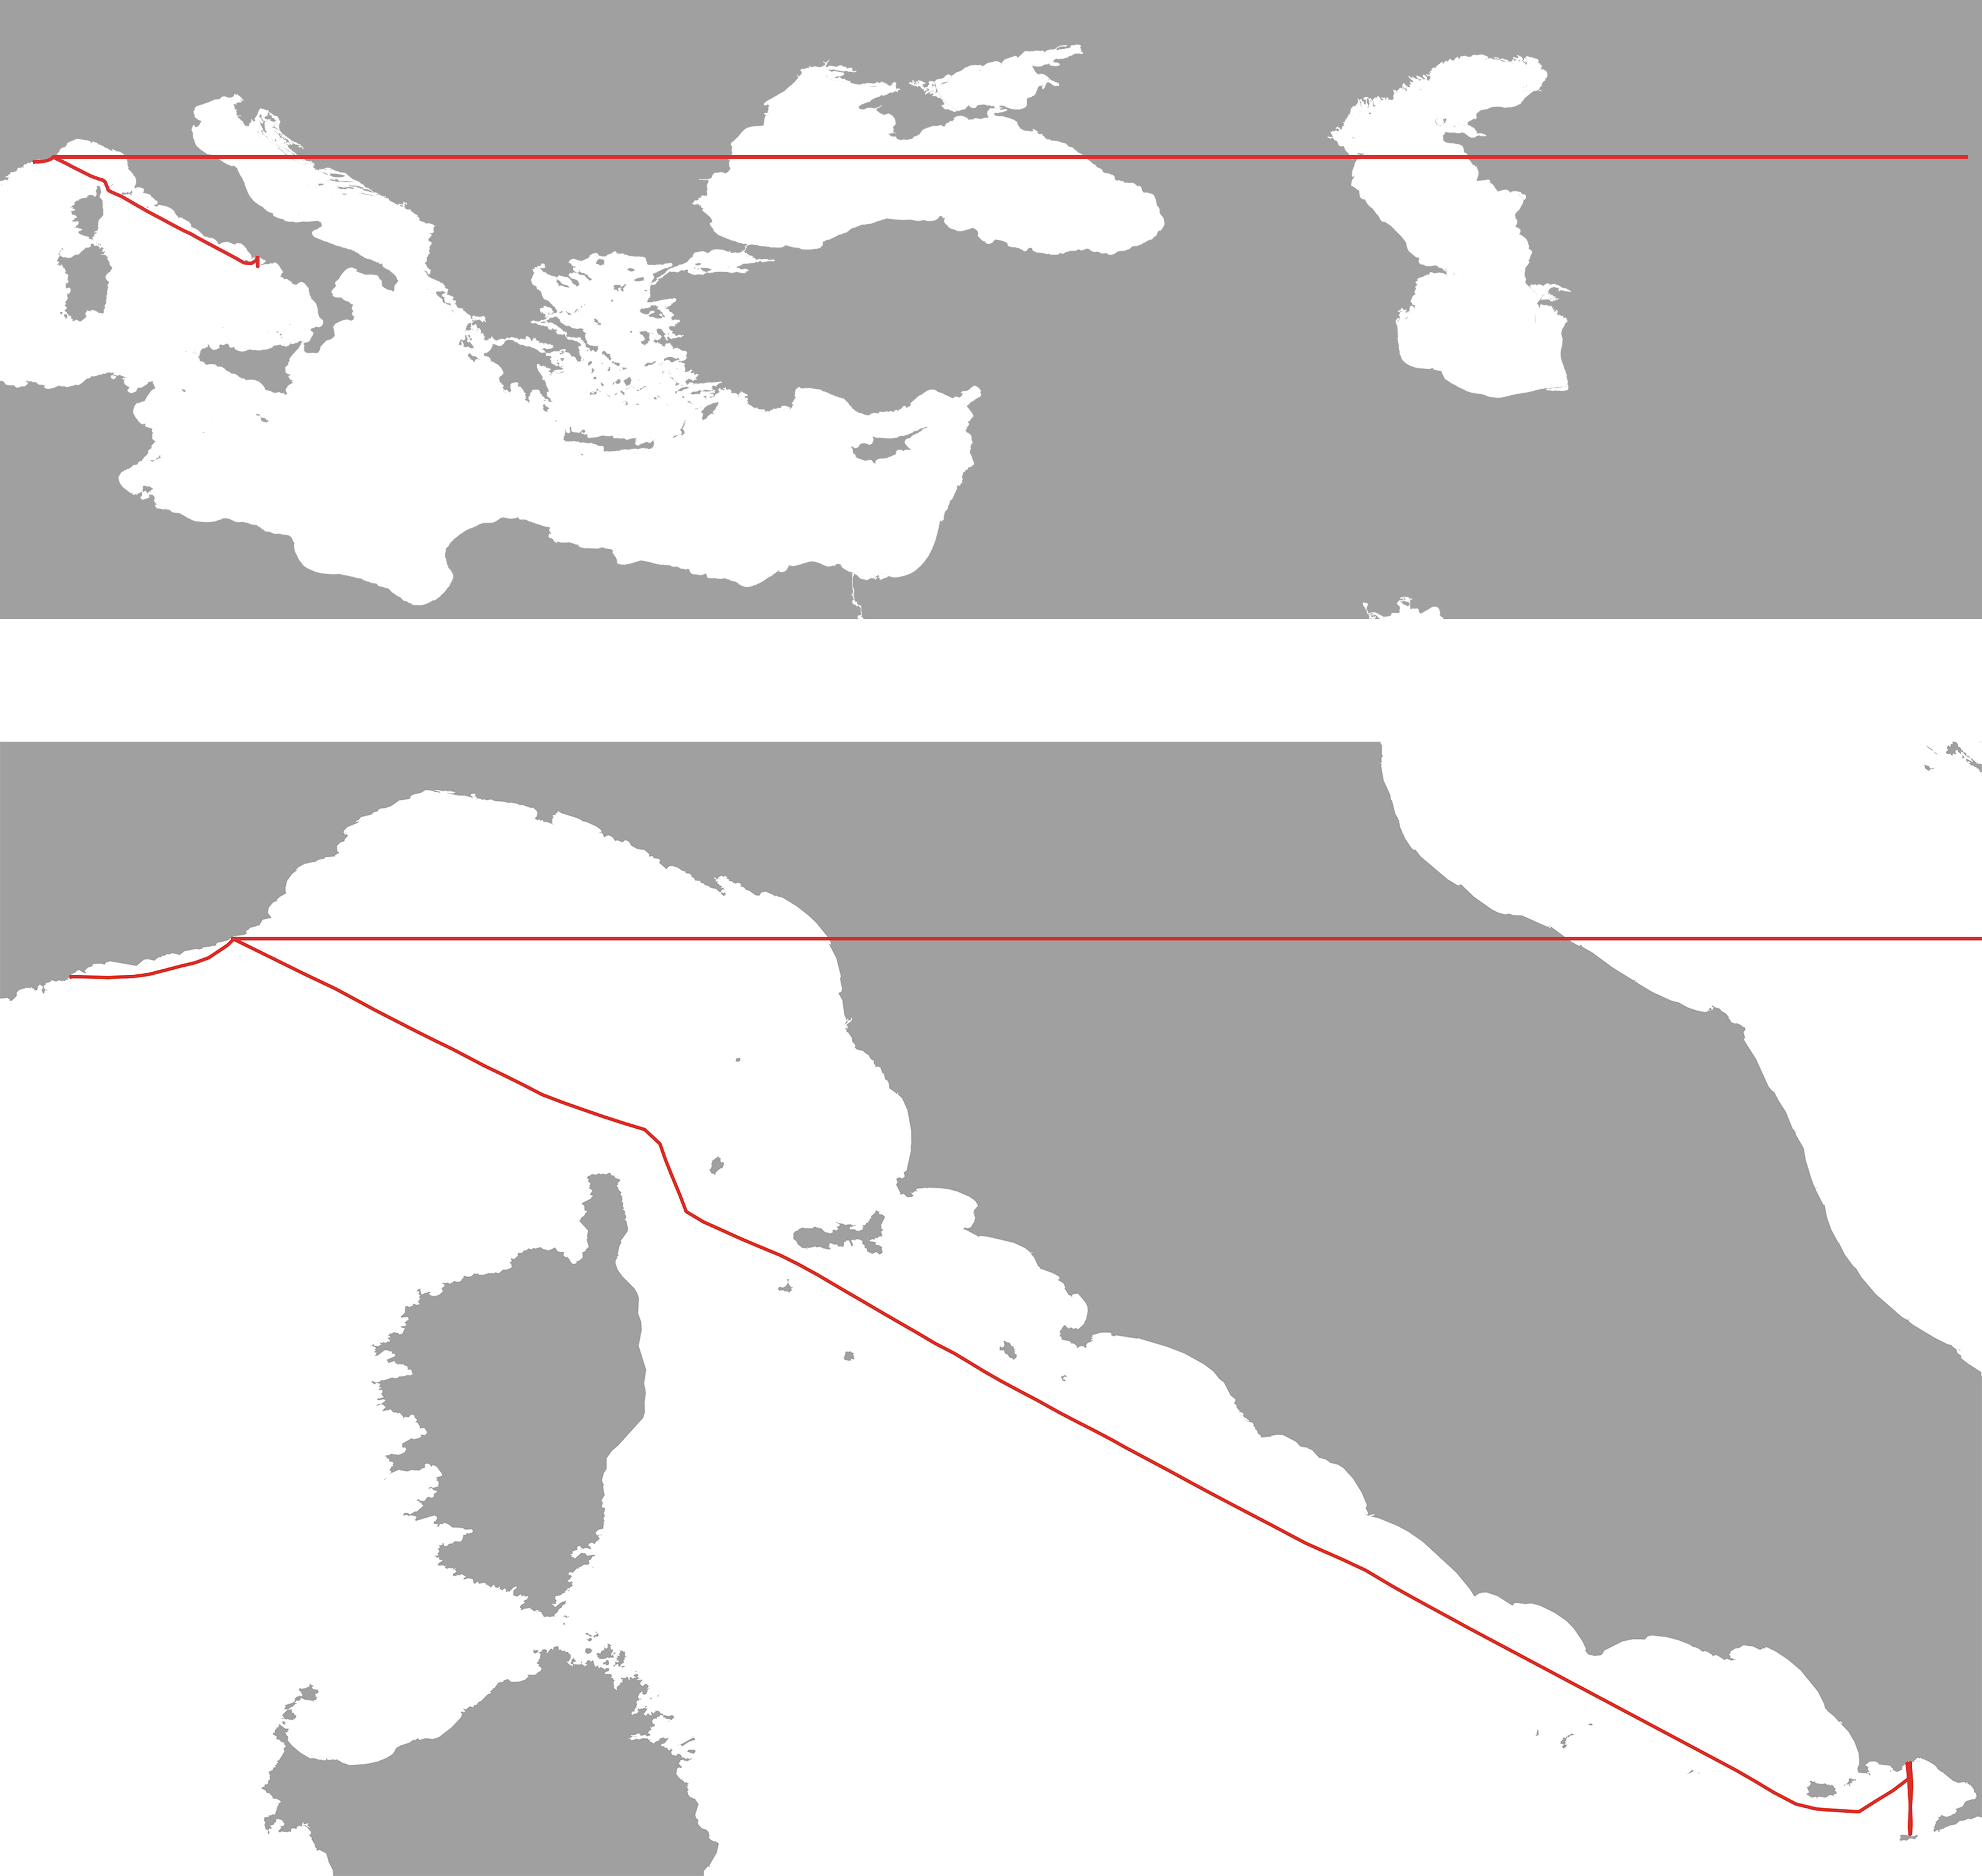
\includegraphics[width=0.7\textwidth]{figures/trajectory_noise/noisy_trajectory}
    \caption{Example showing a ``noisy'' trajectory presumably caused by GPS inaccuracy or equipment error}
    \label{fig:noisy_trajectory}
\end{figure}

An example of this issue is visualized in \cref{fig:noisy_trajectory} which shows a voyage starting in Monaco and ending in Naples, Italy. During a stopping point in northern Italy, the vessel transmitted two longitude values placing the vessel in the middle-east while then continuing the journey arriving in Naples, Italy. This issue is presumably caused by issues with the GPS signals sent by the \acrshort{ais} transmitter onboard the vessel or by some other equipment error. Excluding the fluctuated segment of the trajectory, the remaining trajectory is completely valid, thus, if it is possible to remove the invalid part of the trajectory, the remainder could be further used in the analysis. Therefore, ``noise filter'' was employed to detect and cut away fluctuations in otherwise valid trajectories.

\begin{figure}[htbp]  % order of priority: h here, t top, b bottom, p page
    \centering
    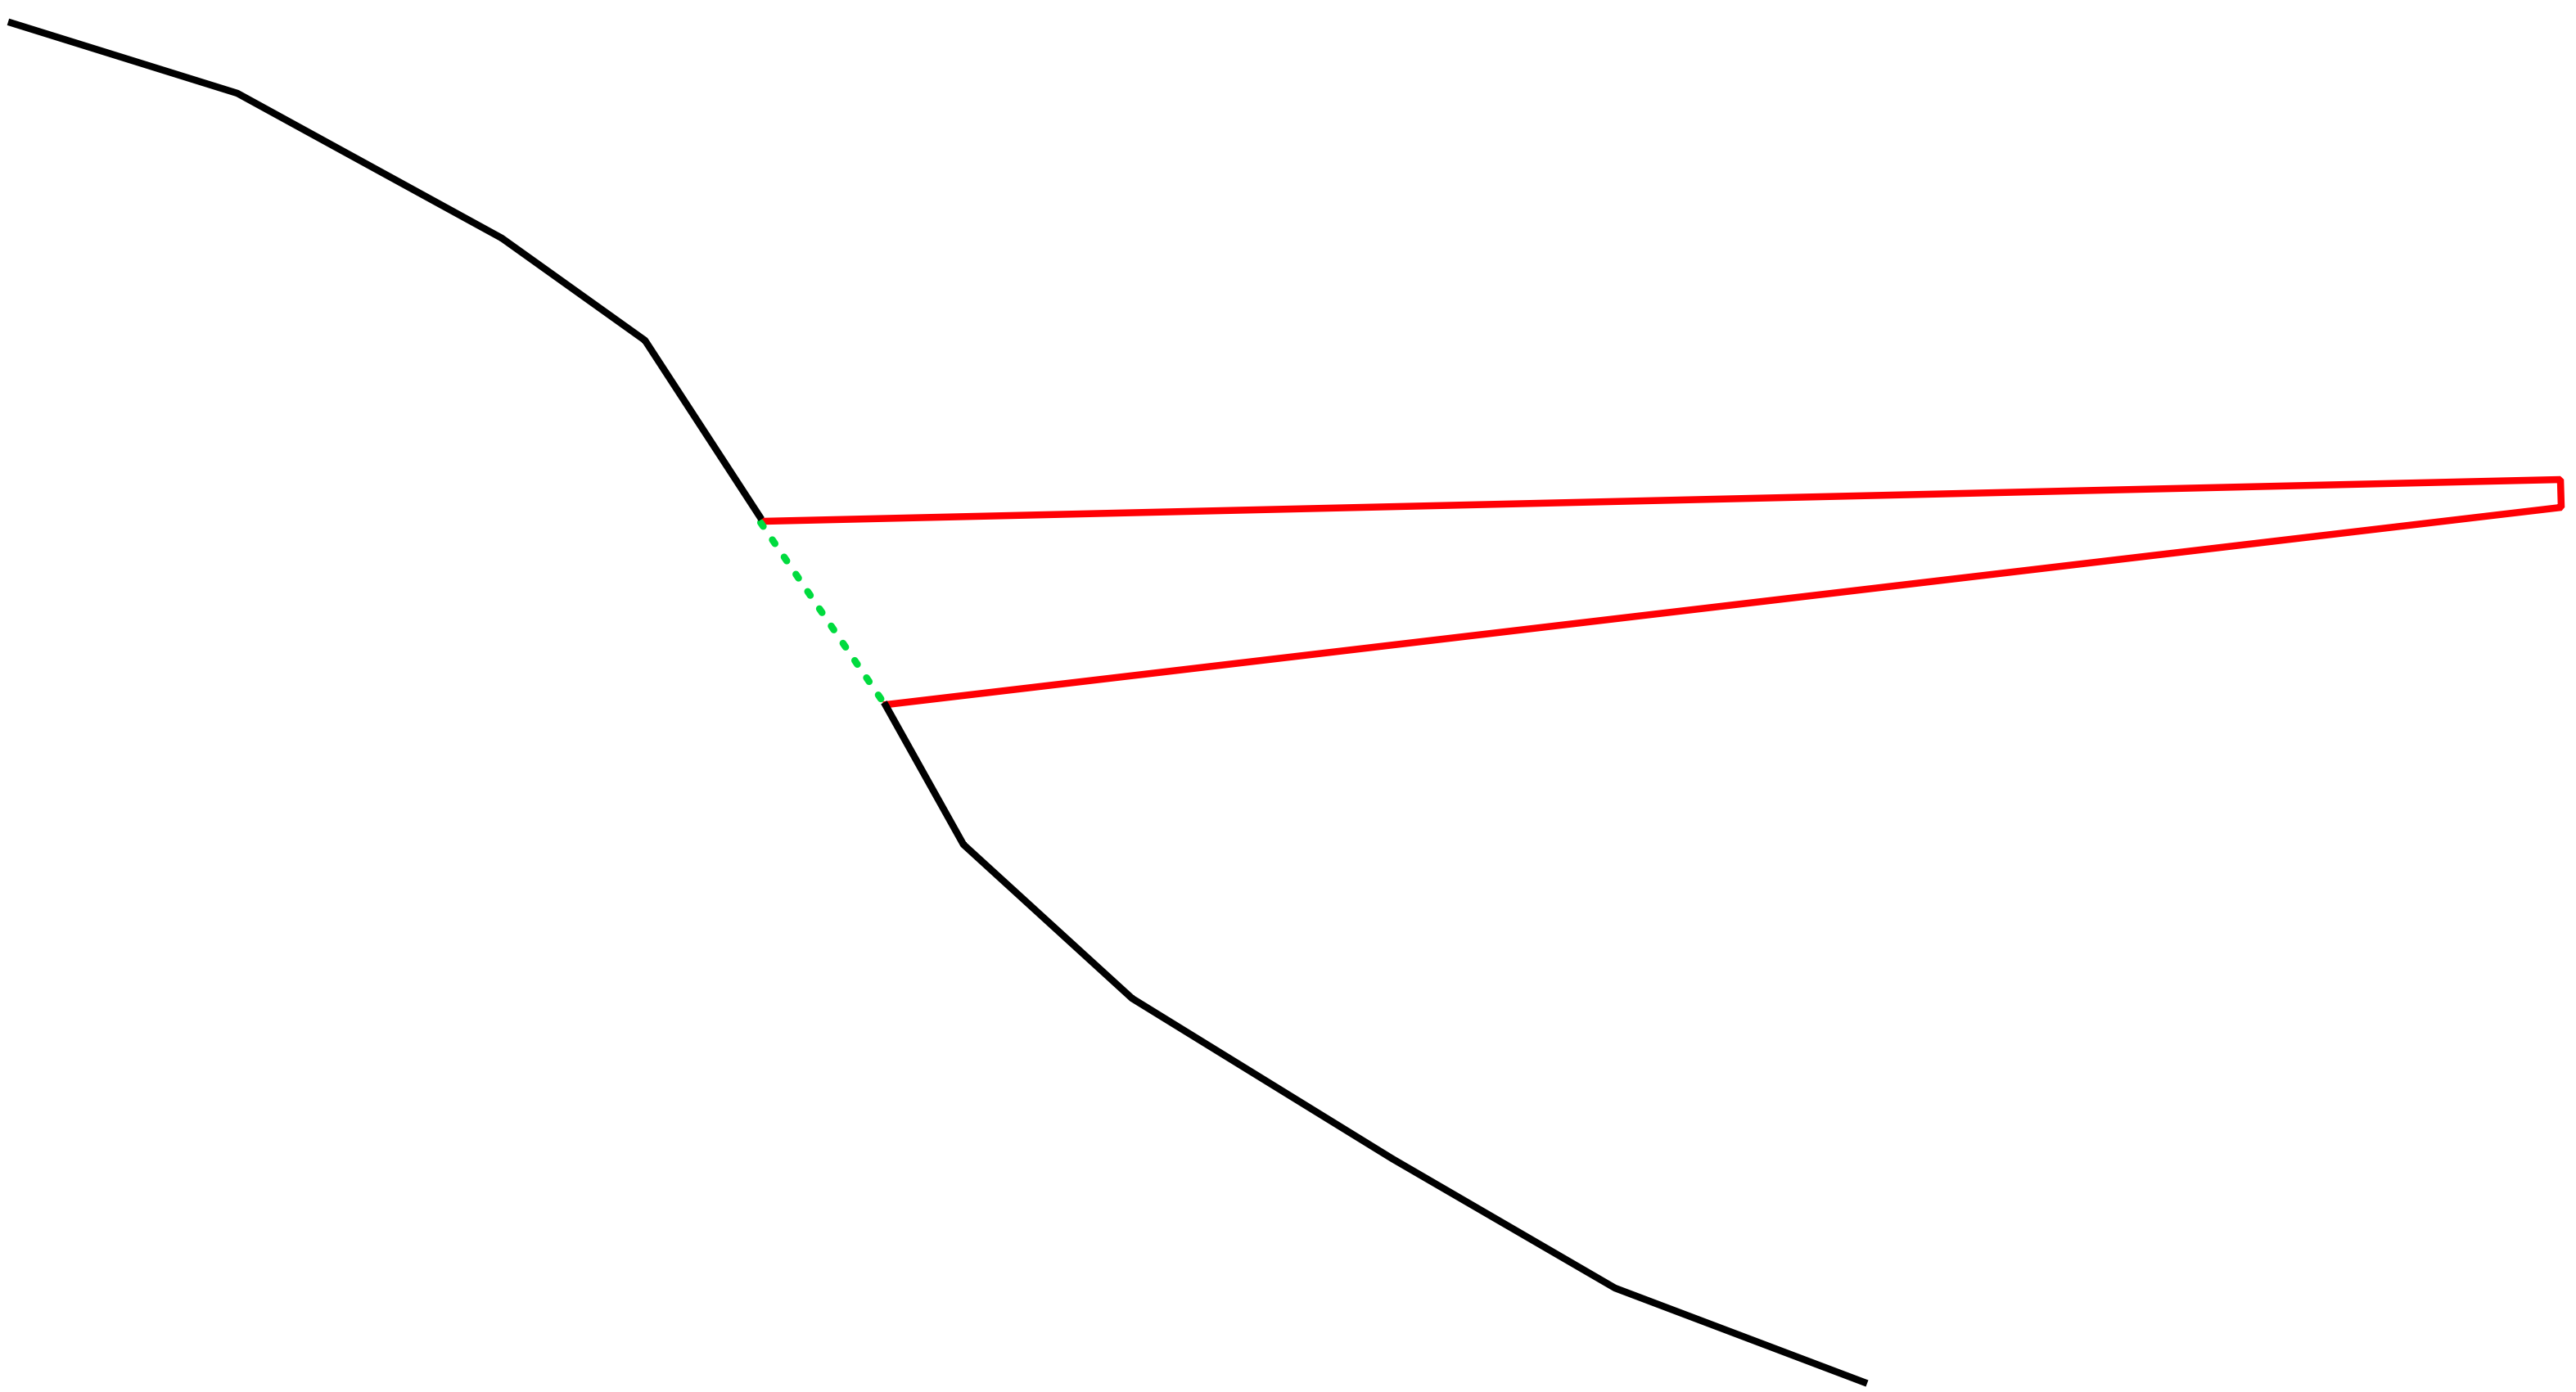
\includegraphics[width=0.6\textwidth]{figures/trajectory_noise/noise_filter}
    \caption{Noise filter algorithm cutting out points in a trajectory detected as noise. The red segment is cut out and the black segments are tied together as shown with the green dotted line.}
    \label{fig:noise_filter}
\end{figure}

\begin{figure}[htbp]  % order of priority: h here, t top, b bottom, p page
    \centering
    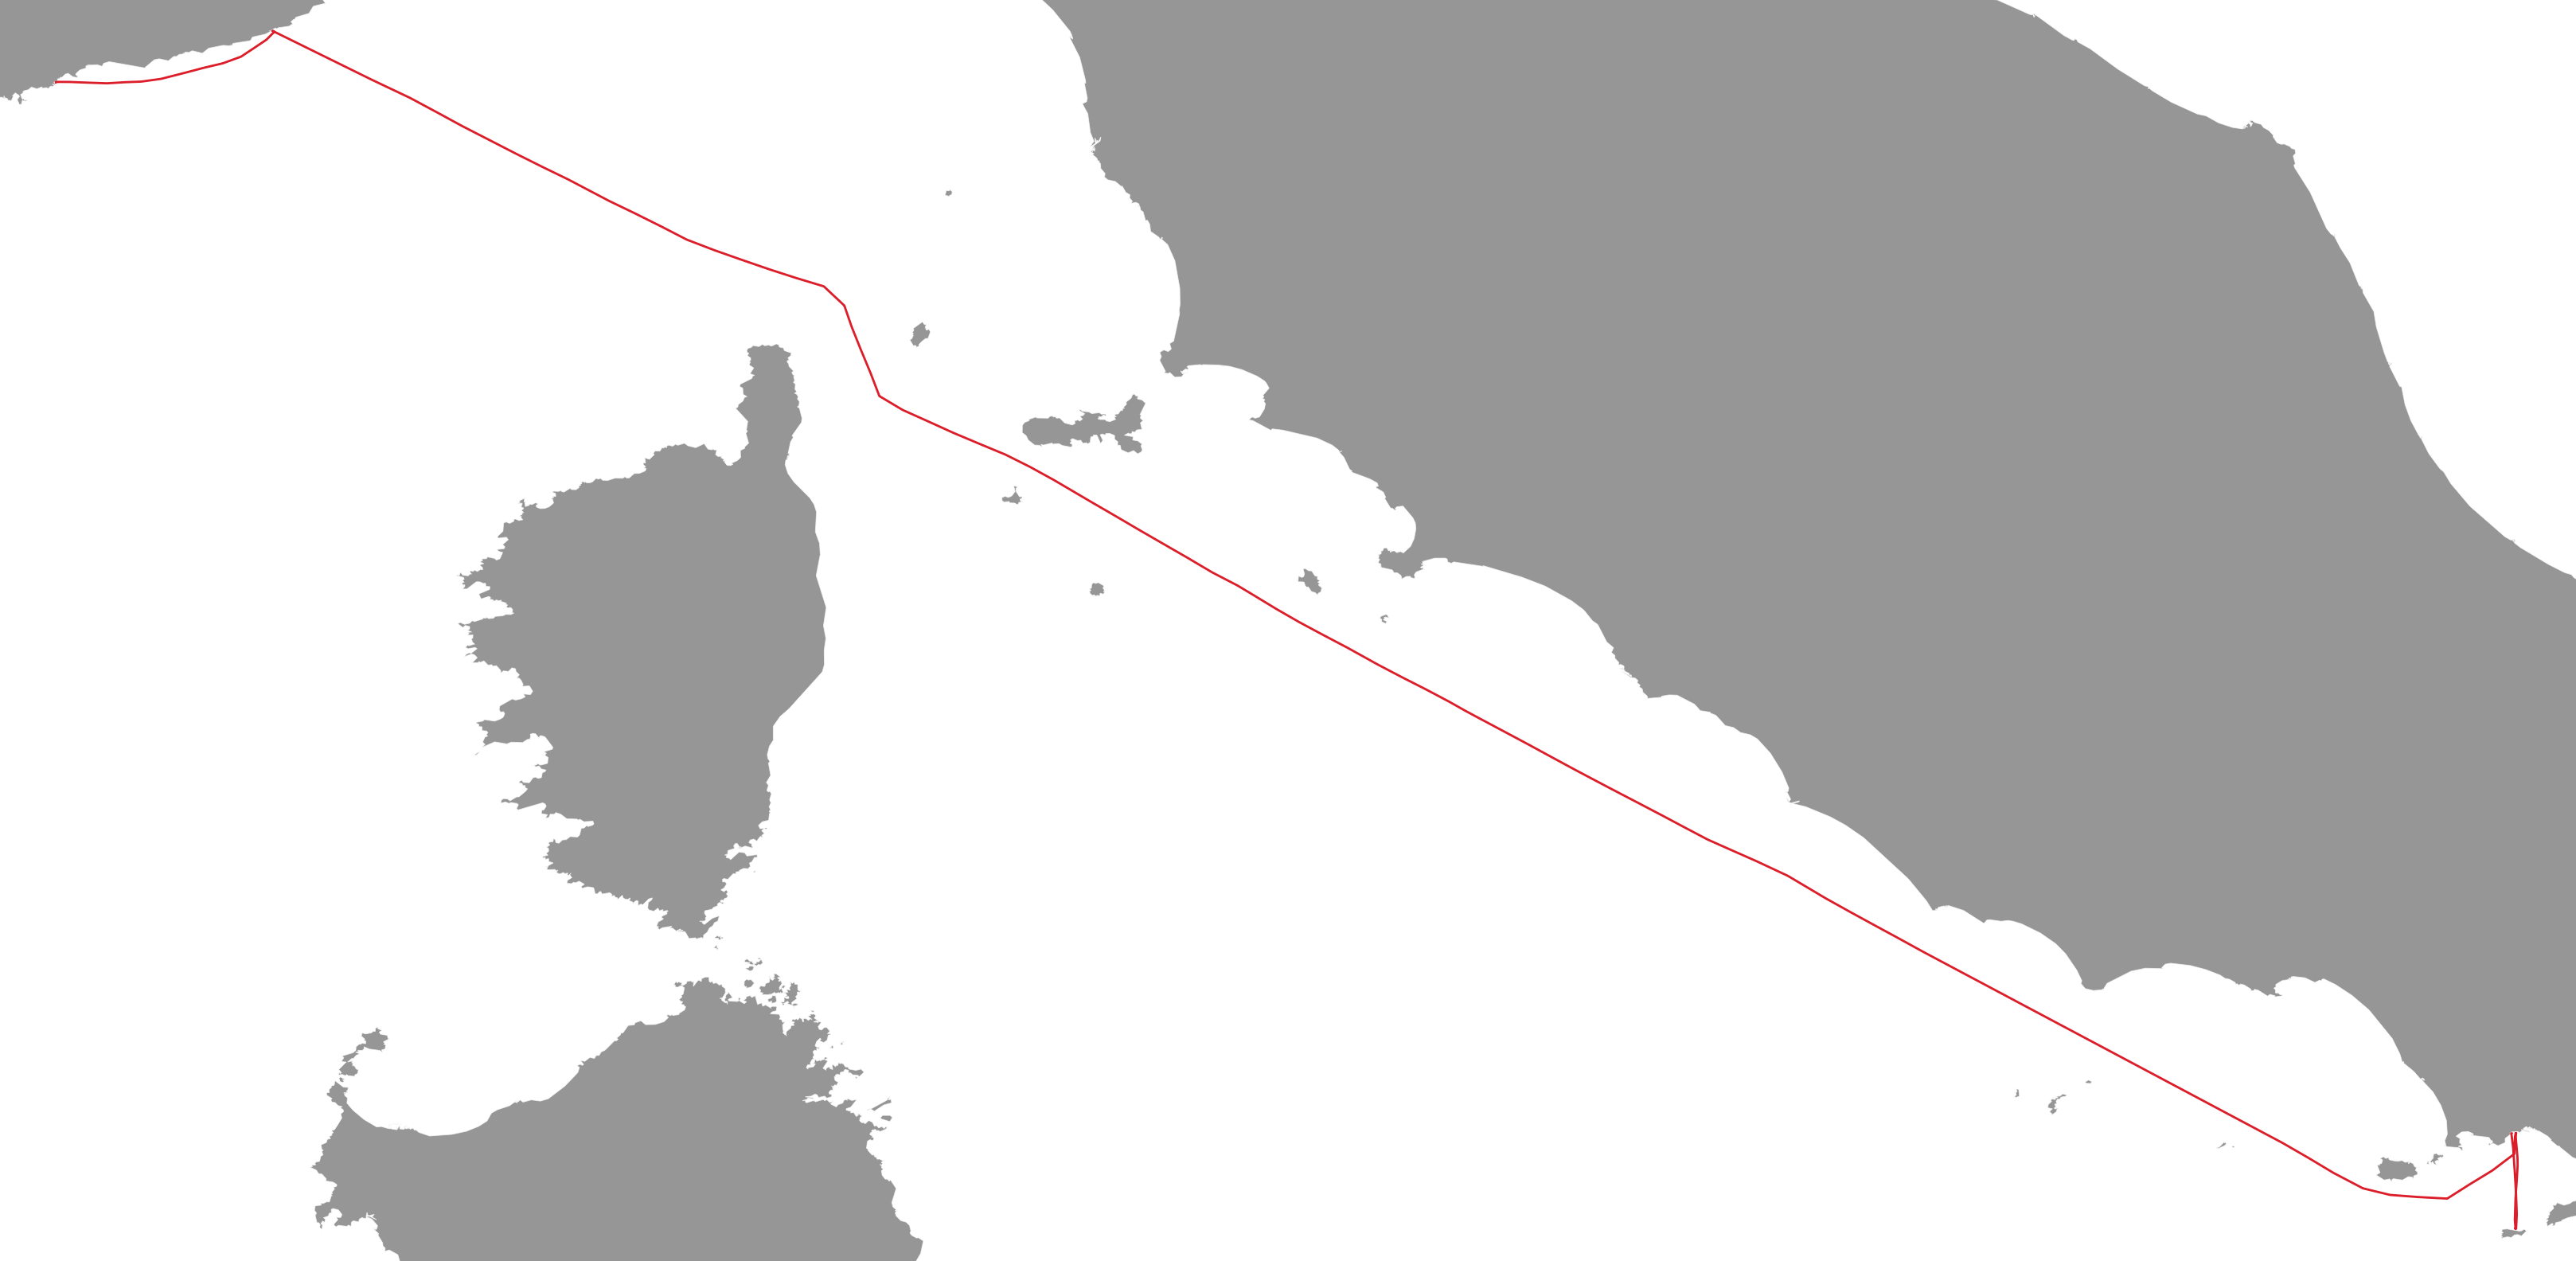
\includegraphics[width=0.8\textwidth]{figures/trajectory_noise/filtered}
    \caption{The example trajectory shown \cref{fig:noise_filter} from Monaco to Naples after noise filtering.}
    \label{fig:noise_filtered}
\end{figure}

The noise filtering employed in the trajectory builder is shown in \cref{fig:noise_filter} where the red segment fluctuates in an otherwise valid trajectory and is therefore excluded from the remaining trajectory. For every point in the trajectory, the algorithm checks the distance between the current and the next point as well as the time difference between the two points. Using the distances in space and time, it calculates the speed the vessel would require to travel from the first to the second point. If the speed required was more than 50 knots, the segment was invalid. The next point is then compared to the first to see if there is a possible valid path to the third point. If there is, the second point is disregarded from the trajectory. The algorithm is given a tolerance of four invalid points before it disregards the entire trajectory. \cref{lst:noise_filter} shows the function used to find the next valid point in a trajectory, if it returns an error, the trajectory is disregarded. \cref{fig:noise_filtered} shows the same trajectory from \cref{fig:noisy_trajectory} after the following algorithm has filtered out fluctuating segments.

\begin{lstlisting}[
    caption={Golang code used find the next valid point for any given point in a trajectory.},
    label=lst:noise_filter,
    language=Go,
    showstringspaces=false,
]
// nextValidPoint returns the index of the next valid point checking distances to
// every point within tolerance. If no valid distances were found wihin tolerance,
// it returns an error. If the last point in trajectory was reached, -1 is returned
func nextValidPoint(start, tolerance int, positions []VesselPosition) (int, error) {
	a := positions[start]
	for j := start + 1; j <= start+tolerance; j++ {
		if j >= len(positions) {
			return -1, nil
		}

		n := positions[j]
		dist := DistanceHaversine(Point{a.Lon, a.Lat}, Point{n.Lon, n.Lat})
		// use the absolute value in case the trajecotory is not sorted
		timeDiff := math.Abs(float64(n.Timestamp - a.Timestamp))

		// calculate the required speed to reach the given point with the
		// given time difference * 1.94385 to konvert m/s to knots
		requiredSpeed := (dist / timeDiff) * 1.94385
		// if required speed was >= 50kt, move on to next point
		if requiredSpeed < 50.0 {
			return j, nil
		}
	}
	// no reasonable distances were found within tolerance
	return -1, errors.New("trajectory segment too noisy")
}
\end{lstlisting}

Finally, when the voyage trajectories have been constructed and validated, they are collected in a database table called transition voyages which contains the following relevant attributes:

\begin{itemize}
    \item imo - an identifier for the vessel.
    \item mmsi - an identifier for the vessel.
    \item departure port - voyage departure port's locode.
    \item departure timestamp - the time of departure.
    \item arrival port - voyage arrival port's locode.
    \item arrival timestamp - the time of arrival.
    \item trajectory - 3D linestring with longitude, latitude, and timestamp for each point.
\end{itemize}

It is worth noting that the trajectories are stored as 3D PostGIS linestring geometries where each point contains an \textit{x}, \textit{y}, and \textit{z} value where the \textit{z} value holds the UNIX timestamp of the positional record. Keeping the timestamp value is necessary for sampling trajectories based on time, and keeping the time values stored directly in the trajectory geometry saves an extra table for trajectory points.

\section{Data processing for \acrfull{ml}}

After the initial data set has been collected and vessel voyages have been defined and constructed, the next step is to build the final training dataset to be used for analysis and \acrfull{ml}. This section describes every step in the process used to construct this dataset based on data described up to this point in this chapter.

\subsection{Trajectory sampling}

Vessels transmit \acrshort{ais} records at different frequencies and messages collected via satellite are collected at different frequencies as the satellites have different orbits. Therefore the frequency, or density, or records in trajectories can not be expected to be standardized. Furthermore, as vessels travel at different speeds, two trajectories with similar start and end positions might have different shapes and contain a different number of points. In addition, as discussed in \cref{sec:vessel_voyage_definition}, one disadvantage of relying on \acrshort{ais} navigational statuses is that vessels can stop during a voyage for different reasons before arriving at their final destinations. Whenever a vessel stops moving or moves slowly, many \acrshort{ais} records are transmitted in clusters which cause noise and redundant data in the constructed trajectories.

\begin{figure}[htbp]  % order of priority: h here, t top, b bottom, p page
    \centering
    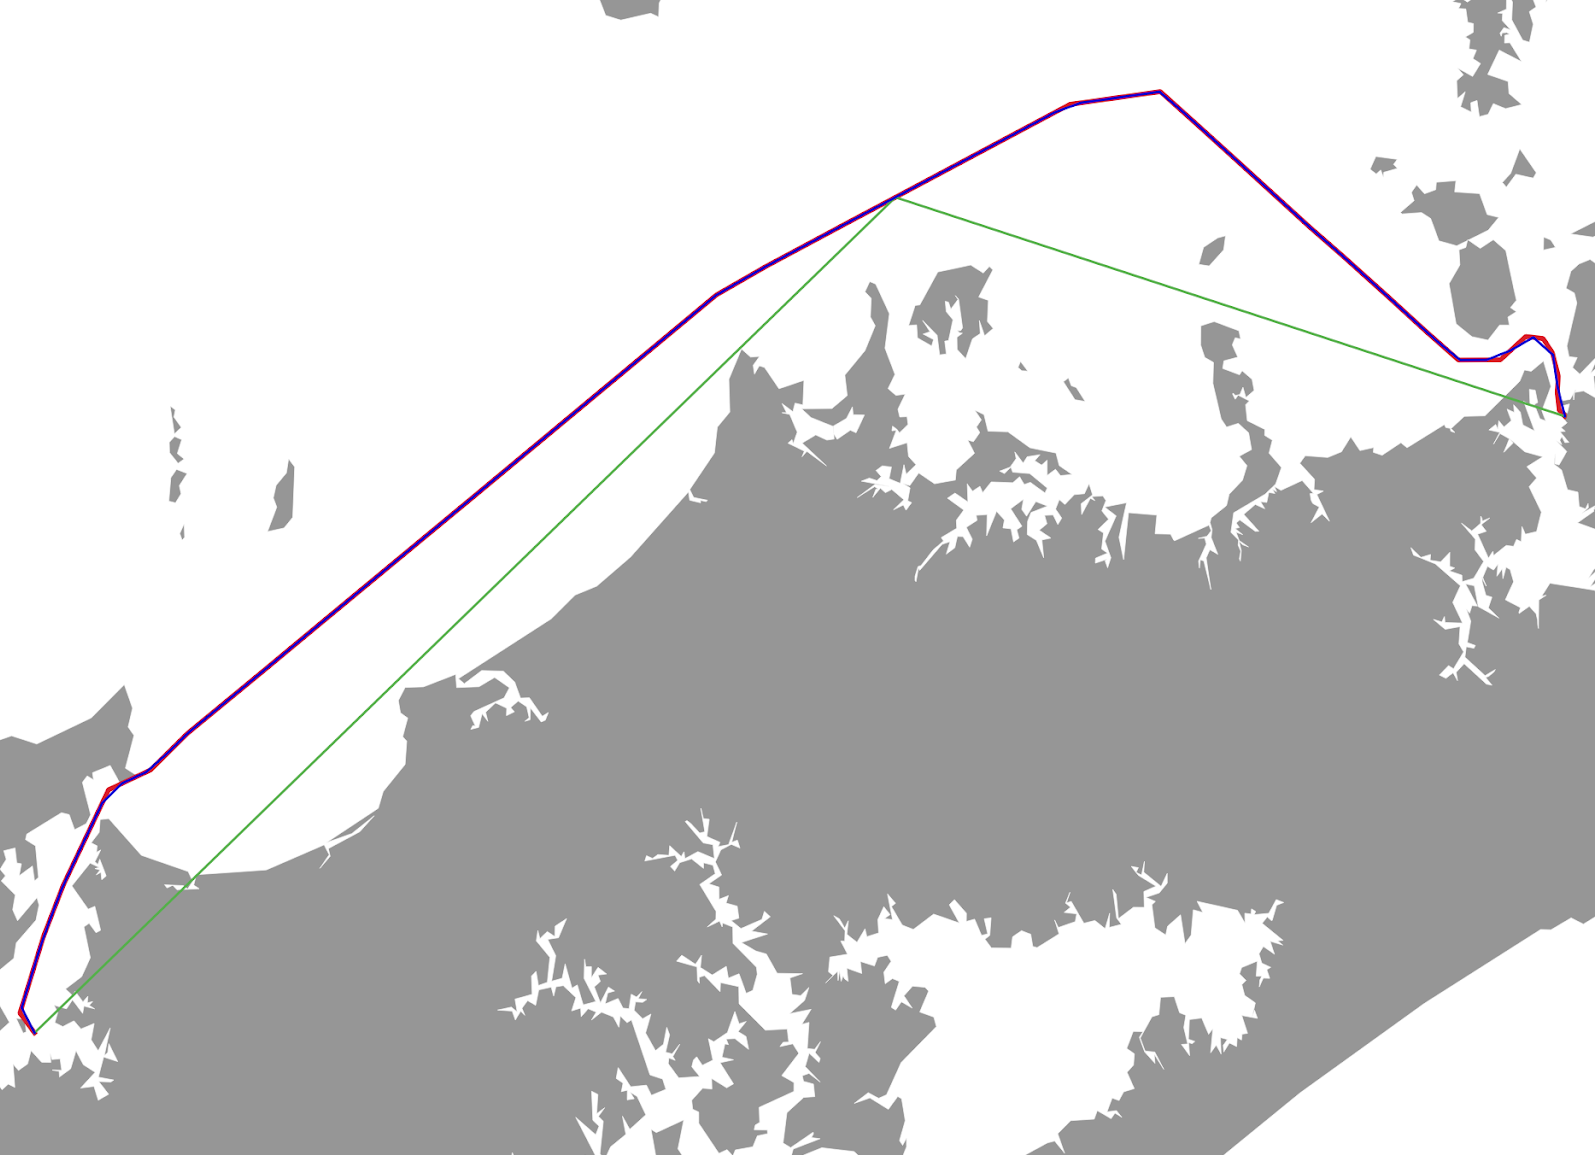
\includegraphics[width=0.8\textwidth]{figures/trajectory_sampling}
    \caption{Example of a trajectory sampled by both distance (2 km) and time (6 hours). The red trajectory is not sampled, the blue is sampled based on 2 km in distance, and the green is sampled based on six hour time intervals.}
    \label{fig:trajectory_sampling}
\end{figure}

The proposed solution includes using similarity between trajectories to predict traveling vessels' destination ports, therefore, in order to make the trajectories more comparable, a sampling step was added in the process of constructing the training data. There were two main approaches considered for trajectory re-sampling, namely sampling based on distance and time. When sampling based on a predefined distance, each subsequent point in a trajectory must be the same distance apart from the next. When sampling based on time, one position is extracted from a trajectory for every given unit of time. For instance, if sampling based on time with a six-hour sample rate, starting from the first point, every position within six-hour intervals is grouped and all positions within each group are dropped except for the first one. Both methods achieve the goal of making trajectories more comparable, however, sampling based on time simplifies, or reduces, the amount of data in each trajectory the most. It also provides an indication of trajectory duration implicitly through the trajectory length or the number of points in a trajectory.

For these reasons, throughout the rest of the implementation, sampling is done based on the time using a time interval of six hours. It is worth noting that for trajectories shorter than six hours, only the first and last point in the trajectory is returned reducing the trajectory to a straight line. In order to sample any trajectory based on either time or distance, a Golang package was written called ``sampler'' which can parse and handle both 3D trajectories including timestamps for time sampling and 2D trajectories for distance sampling. The complete code for this package can be found in \cref{app:sampler}. \cref{lst:trajectory_sampler} shows an extract from this package of the function used to resample trajectories based on time.

\begin{lstlisting}[
    caption={Golang code from a sampler package written to sample a trajectory based on time.},
    label=lst:trajectory_sampler,
    language=Go,
    showstringspaces=false,
]
// resampleTime resamples trajectory based on s.SampleRate given in hours.
// Extracts the first position within intervals based on sample rate
func (s *Instance) resampleTime() (string, error) {
	var err error
	trajectory, err := s.parse3DTrajectory()
	if err != nil {
		return "", err
	}

	intervals := s.getTimeIntervals(trajectory)
	reducedCoords := []geom.Coord{}
	coords := trajectory.Coords()

	// within each interval add the first coord to reducedCoords
	for _, interval := range intervals {
		var first *geom.Coord

                // get first coord in interval
		for i := range coords {
		        // roundTime uses s.SampleRate when rounding
			coordInterval := s.roundTime(int64(coords[i][2]))
			if coordInterval == interval {
				first = &coords[i]
				break
			}
		}
		if first != nil {
			reducedCoords = append(reducedCoords, *first)
		}
	}

	// if the last coord wasn't the last in reduced, add it
        lastReduced := reducedCoords[len(reducedCoords)-1]
	if !lastReduced.Equal(geom.XYZ, coords[len(coords)-1]) {
		reducedCoords = append(reducedCoords, coords[len(coords)-1])
	}
	if len(reducedCoords) <= 1 {
		return "", errors.New("too few points in sampled trajectory")
	}
	reduced, err := geom.NewLineString(geom.XYZ).SetCoords(reducedCoords)
	if err != nil {
		return "", err
	}

	return geomwkt.Marshal(reduced)
}
\end{lstlisting}

The function listed in \cref{lst:trajectory_sampler} is used in a batch process that samples every voyage's trajectory and keeps the sampled voyages in a separate table called ``sampled transition voyages''. The batch process extracts 5000 voyages at a time, samples their trajectories, and batch-inserts them into a separate table. By not mutating the original voyage data, different sampling methods can be applied and tested to find differences in trajectory comparisons. The final structure of the sampled transition voyages database table is described in \cref{tab:sampled_voyages}

\begin{table}[htbp]
    \centering
    \small{\begin{tabularx}{1.0\textwidth}{p{1.3in} p{0.75in} X}
        \bfseries{Column} & \bfseries{Type} & \bfseries{Description} \\ \toprule
        voyage\_id & int & reference to the original voyage id \\ \midrule
        imo & int & identifier for the traveling vessel\\ \midrule
        mmsi & int & identifier for the traveling vessel\\ \midrule
        departure\_port & string & \gls{locode} of the vessel's departure port \\ \midrule
        departure\_timestamp & int & Unix timestamp from when the vessel departed the departure port \\ \midrule
        arrival\_port & string & \gls{locode} of the vessel's arrival port \\ \midrule
        arrival\_timestamp & int & Unix timestamp from when the vessel arrived at the arrival port \\ \midrule
        trajectory & geometry & 3D linestring with longitude, latitude, and timestamp for each point \\ \bottomrule
    \end{tabularx}}
\caption{Structure of the ``sampled\_transition\_voyages'' table.}\label{tab:sampled_voyages}
\end{table}

\subsection{\acrfull{mstd}}

In order for the proposed solution to take into account both geographical trajectories as well as additional vessel information for predictions, in the training set, the trajectories have been abstracted into the categorical and numeric values \acrfull{mstd}, the similarity value for the \acrshort{mstd}, and then the length of the trajectory. The \acrshort{mstd} value is essentially an initial prediction of the vessel's final destination purely based on geographical, or spatial, trajectories. This is similar to other approaches found in other studies such as \cite{Zhang2020AISApproach}. Purely spatial trajectory predictions works quite well when the trajectories are complete, or close to the vessels' final destination, however, when a vessel has just recently departed a port for a long voyage, there are many possible destination ports and routes the vessel might take. The closer the vessel is to its final destination, the fewer possible candidate ports are there. When considering short trajectories of recently departed vessels, the most similar historical trajectory is not likely to be a good estimation of where the vessel is traveling to. In these cases, relying on more general traveling patterns seem more appropriate. For example, the vessel's departure port, segment, and sub-segment are likely to be much better indicators as to the vessel's final destination. Therefore, the \acrshort{mstd} is only part of the final dataset used for predictions.

The \acrshort{mstd} for a given voyage is found by measuring the similarity between the given voyage's trajectory and every historical trajectory in the sampled transition voyages table. The most similar trajectory is found using a given trajectory similarity measurement, and its destination and similarity value is added to the final dataset. As described in \cref{sec:trajectory_similarity}, there are several different trajectory similarity measurements available, however, for this thesis the \acrfull{sspd} is used to calculate the \acrshort{mstd} values. However, the process and the dataset are structured in such a way that it is possible to use different similarity measurement methods in this process. For instance, the \acrshort{ml}-based method proposed \cite{Zhang2020AISApproach} achieved good performance for similarity-based predictions, thus it could be replicated and used to calculate the \acrshort{mstd} values for this approach.

\begin{figure}[htbp]  % order of priority: h here, t top, b bottom, p page
    \centering
    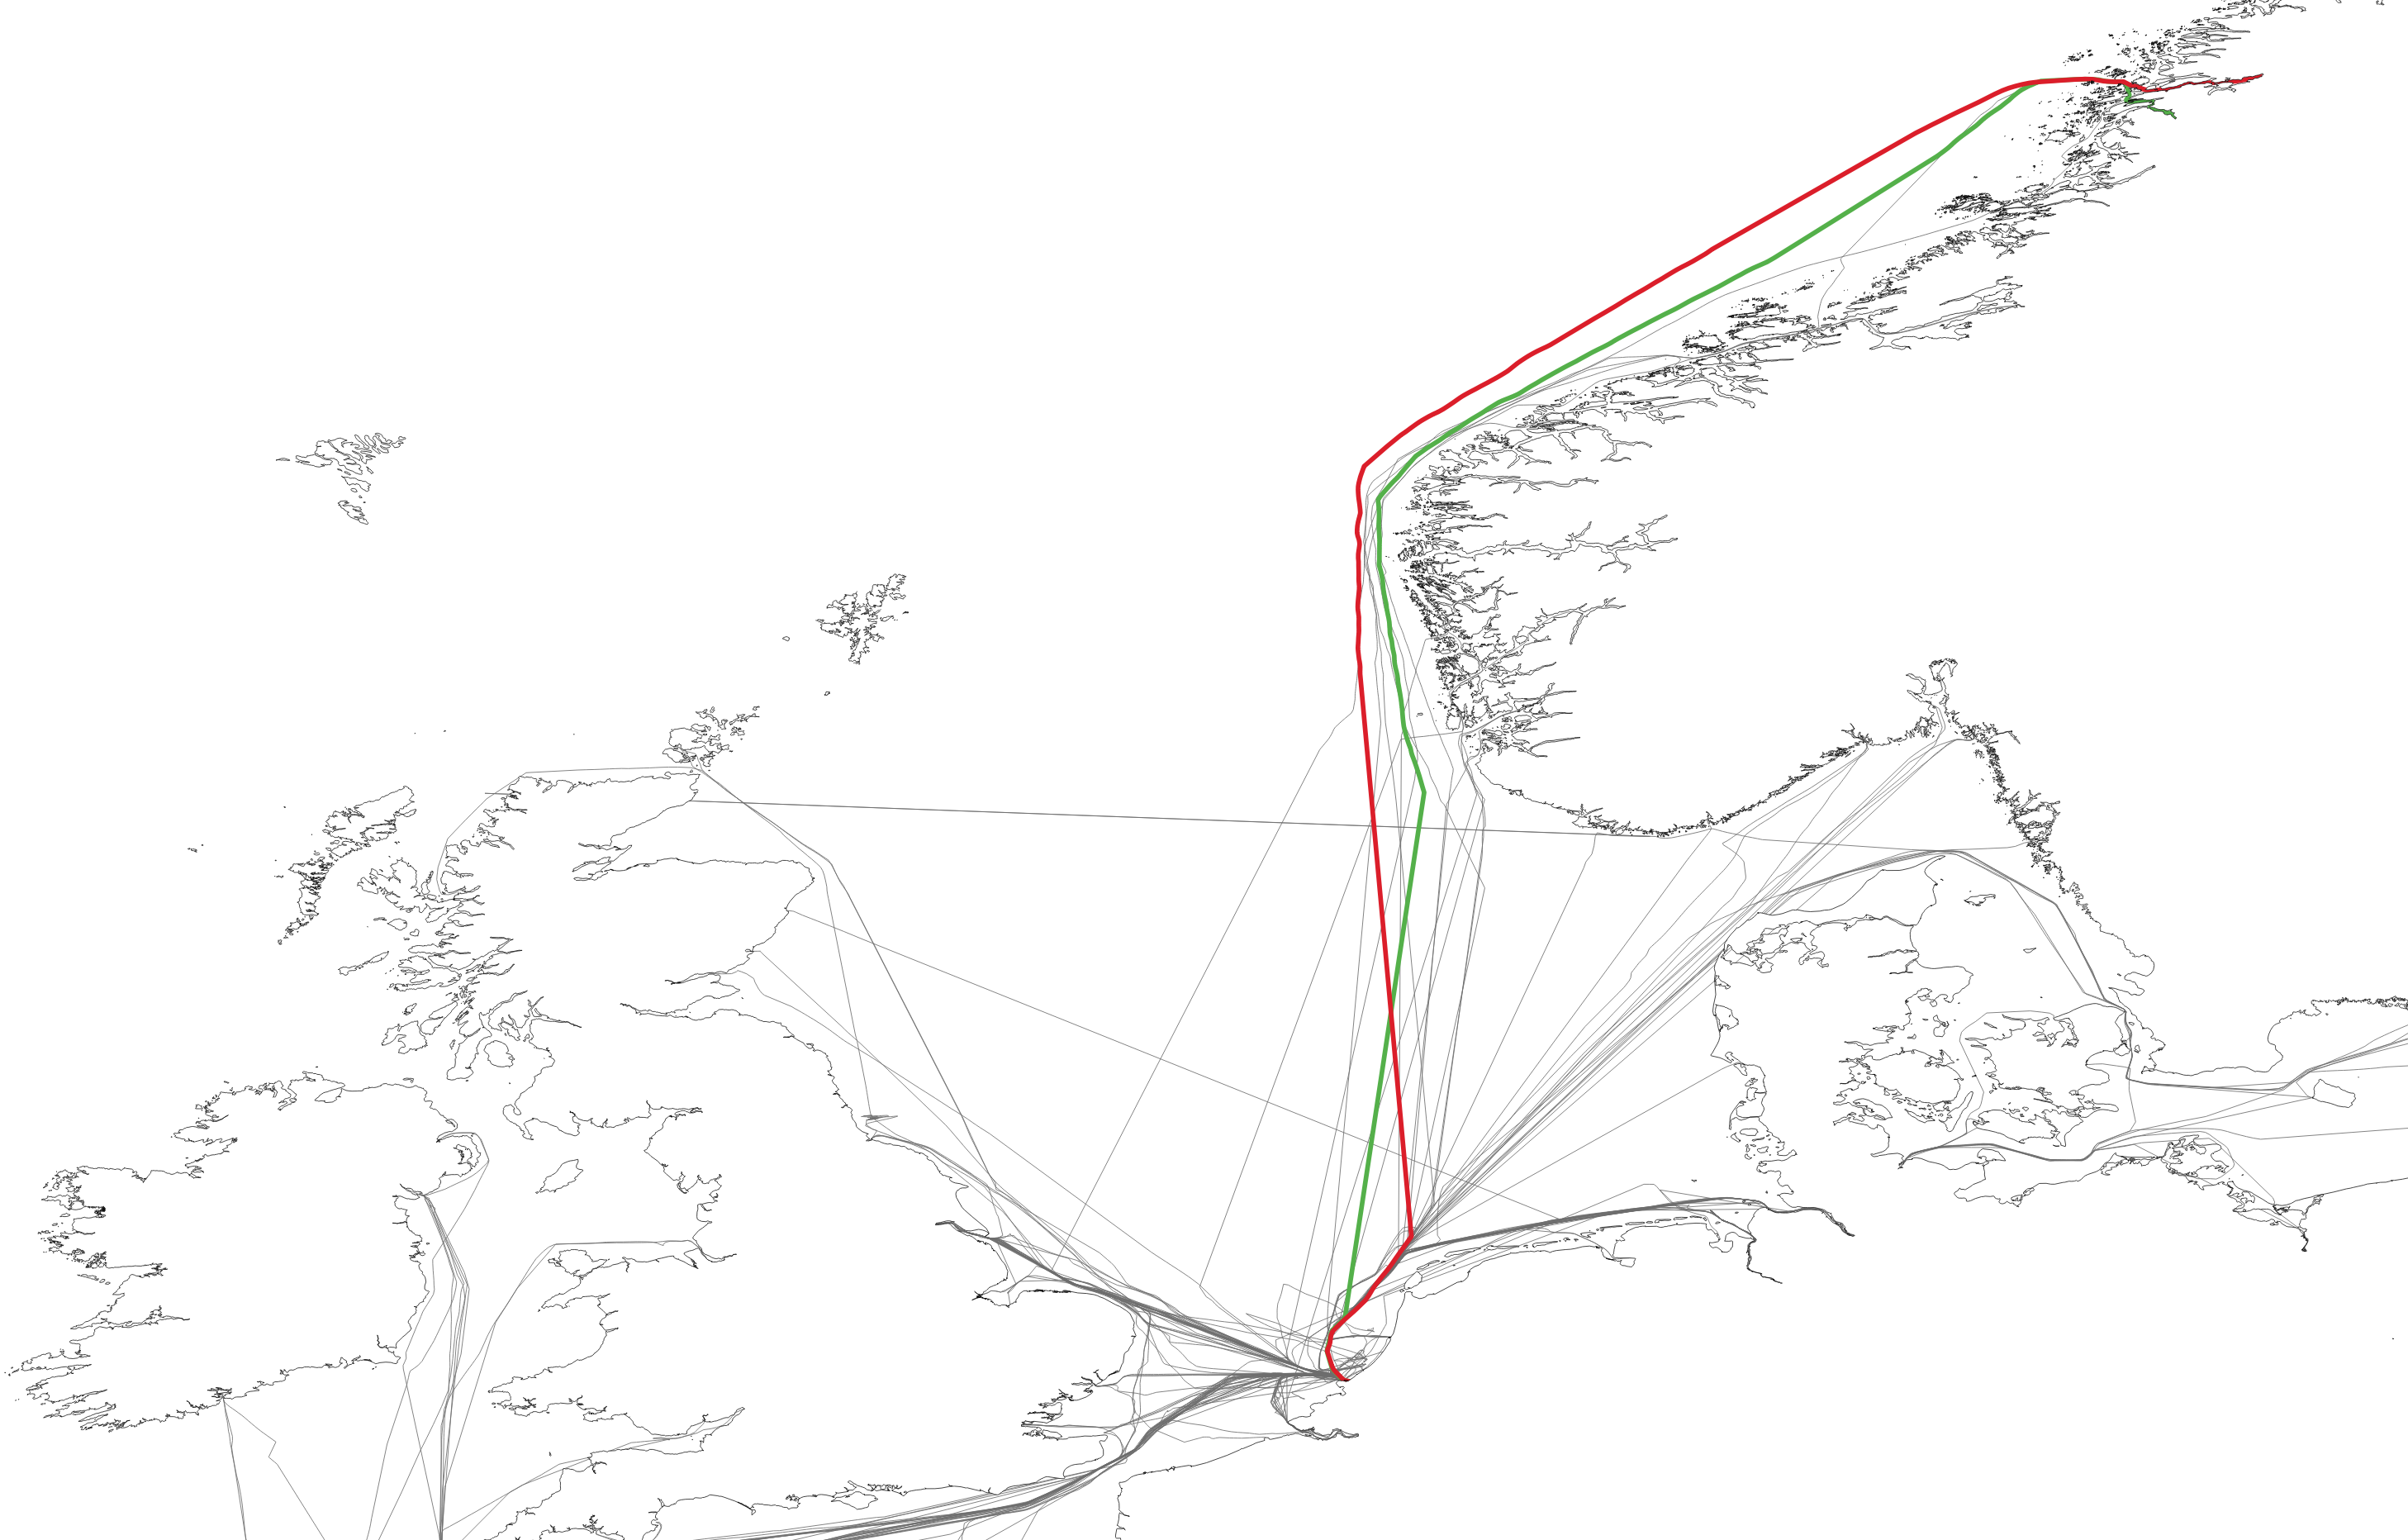
\includegraphics[width=1.0\textwidth]{figures/mstd}
    \caption{Example of \acrshort{mstd} for a given historical trajectory where the red line is the given trajectory and the green line is the most similar historical trajectory.}
    \label{fig:mstd}
\end{figure}

The \acrshort{mstd} value for a given voyage is calculated in the following steps:

\begin{enumerate}
    \item Given a sampled voyage, fetch every historical voyage with the same departure port from vessels of the same segment and sub-segment.
    \item Use a given similarity measurement method, \acrshort{sspd} in this case, to calculate the similarity between the given voyage's trajectory and every historical voyage's trajectory. The given similarity measurement method must return a similarity value. For \acrshort{sspd}, this value is a Haversine distance value.
    \item Find the most similar historical trajectory or the trajectory with the smallest similarity value.
    \item Extract the most similar historical trajectory's destination port as the \acrshort{mstd} value and extract the similarity value for future use.
\end{enumerate}

\cref{fig:mstd} shows an example of finding the most similar historical trajectory (green line) for a given voyage (red line). The given voyage departed the port of Rotterdam and arrived in Mo i Rana, Norway. Every other historical voyage that departed Rotterdam from vessels of the same segment and sub-segment was then extracted and \acrshort{sspd} was used to find the most similar historical trajectory.

\subsection{Building ML data training set}

After the data has been collected, and the \acrshort{mstd} method has been implemented to translate geographical trajectories into categorical and numerical values, the last step is to collect data attributes from the initial data foundation and to calculate \acrshort{mstd} values for every historical trajectory. The final dataset is used to train a \acrfull{ml} model that aims to predict the arrival port of voyages based on these values. Furthermore, to ensure that the training data is reflective of real-life scenarios, the full historical trajectories were divided into several incomplete voyages when calculating \acrshort{mstd} values. This ensures that the final model is able to predict the arrival port of traveling vessels before they reach their final destination. Thus, the process of constructing the final training dataset can be summarized in the following steps:

\begin{enumerate}
    \item Extract the values listed in \cref{tab:sampled_voyages} from the sampled voyages.
    \item Divide the trajectory up to four different smaller trajectories based on the length of the trajectory.
    \item Calculate the \acrshort{mstd} for every trajectory.
    \item Collect the values from each voyage as well as the \acrshort{mstd}, similarity value, and length of the voyage trajectory for the training data.
\end{enumerate}

The process of dividing a trajectory into multiple shorter lengths is relatively straightforward and is shown in \cref{lst:incomplete_voyages}. It is worth noting that trajectories containing less than four points are skipped as the constructed trajectories must have at least two points. Trajectories with exactly four points are divided into two parts instead of four for the same reason.

\begin{lstlisting}[
    caption={Python code used to create incomplete voayges by dividing them into multiple lengths.},
    label=lst:incomplete_voyages,
    language=Python,
    showstringspaces=false,
]
def get_incomplete_trajectories(df, parts=4):
    """divides trajectories in df into n parts

    Given a trajectory of length 8.
    We want to create the following sub-trajectories by incrementing with 8/4=2
     0  1
     0  1  2  3
     0  1  2  3  4  5
     0  1  2  3  4  5  6  7 # original
    """
    ret_df = pd.DataFrame(columns=df.columns)
    for _, r in df.iterrows():
        row = r.copy(deep=True)
        traj = row["trajectory"]
        length = len(traj)

        # we cant make trajectories of length 1
        # so we use half the number of parts
        if length == parts:
            parts = math.floor(parts/2)

        inc = math.floor(length/parts)
        if inc == 0:
            # skip trajectories shorter than parts
            continue

        for i in range(inc, length, inc):
            new_traj = traj[:i]
            if len(new_traj) < 2:
                continue

            row["trajectory"] = new_traj
            row["trajectory_length"] = len(new_traj)
            ret_df = ret_df.append(row, ignore_index=True)
    return ret_df
\end{lstlisting}

As an example, \cref{fig:incomplete_voyage} shows a voyage traveling from China to Argentina. The code listed in \cref{lst:incomplete_voyages} was use to divide the voyage trajectory into four parts that are highlighted by the different colored segments of the trajectory.

\noindent
\begin{figure}[htbp]
    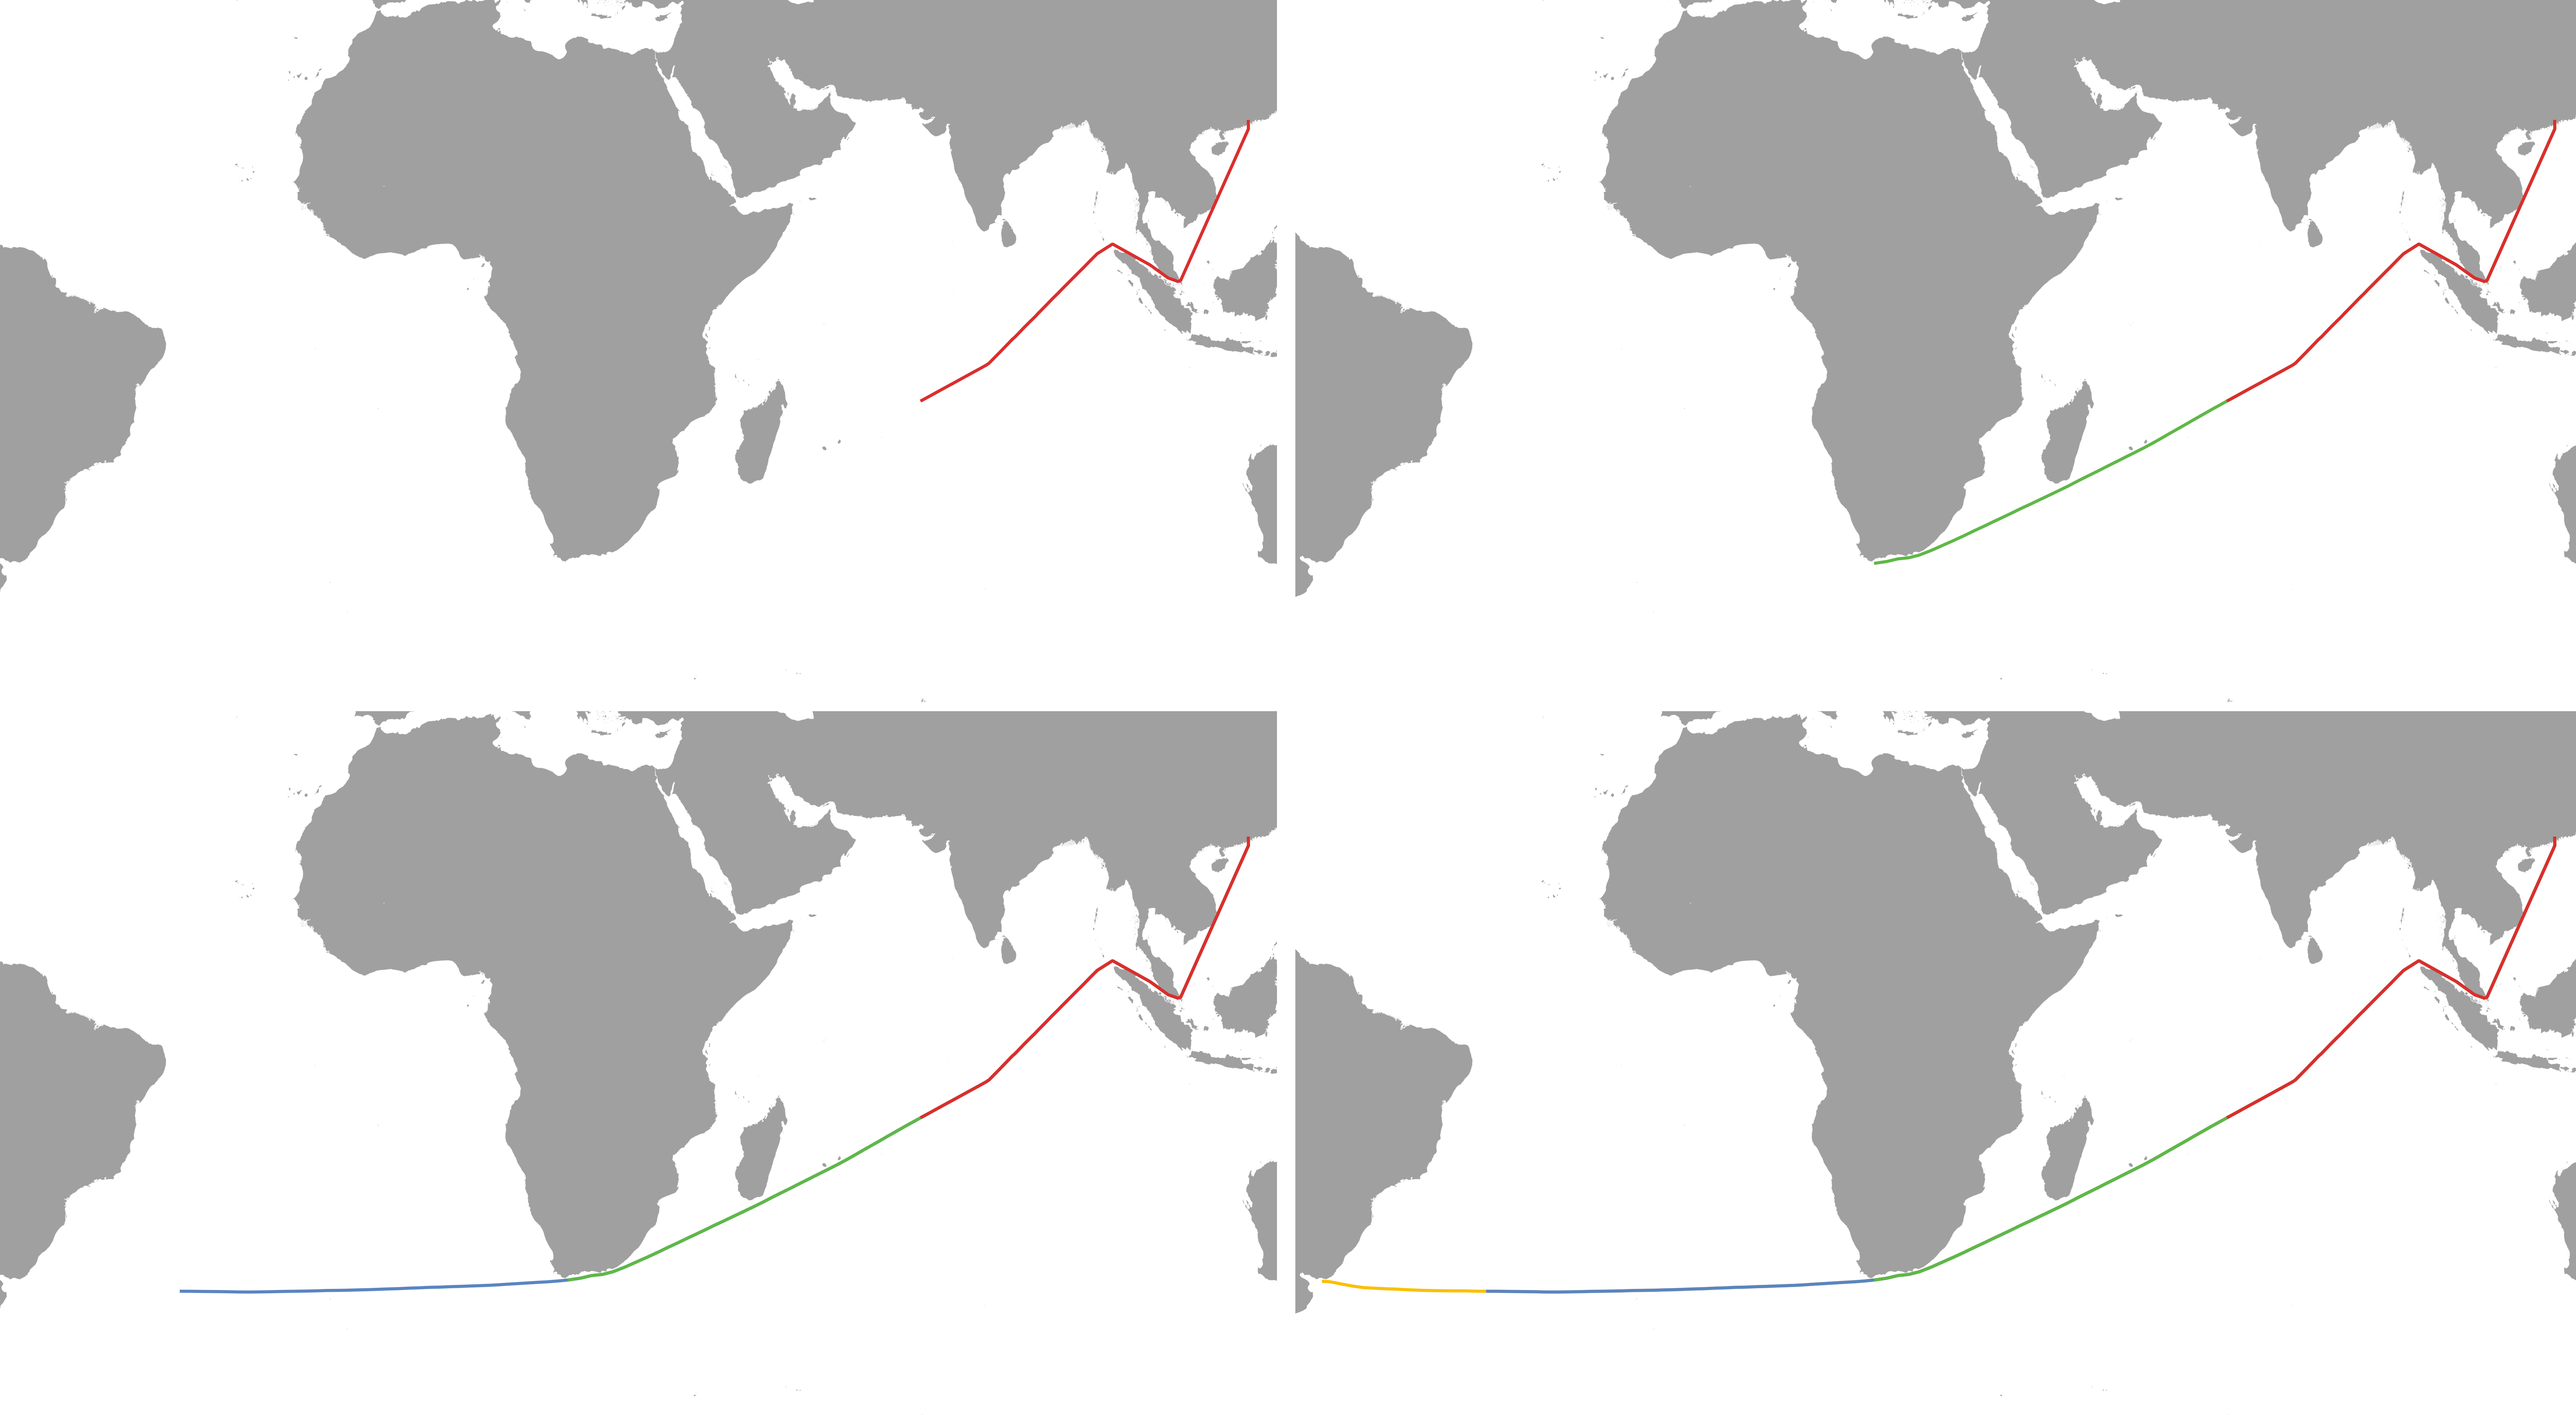
\includegraphics[width=1.0\textwidth]{figures/incomplete_voyage}
    \caption{A voyage (ID 3305) from China to Argentina divided up into four subsets emulating incomplete voyages.}
    \label{fig:incomplete_voyage}
\end{figure}

The similarity value derived from the \acrshort{mstd} calculation and the length of the trajectory is also included in the training set so that a \acrshort{ml} model can find correlating patterns between the length of the trajectory, the similarity value, and the \acrshort{mstd} value. The length of the trajectory indicates how long the vessel has been at sea and thus how close it is to its destination. Therefore, both the trajectory length and the derived similarity value serve as weights for the \acrshort{mstd} value. The expected pattern from the constructed incomplete voyages is exemplified in \cref{tab:incomplete_voyage}. When the trajectories are short and the \acrshort{sspd} distance is high, it should indicate that the \acrshort{mstd} value is more likely to be wrong. When the vessel is closer to the destination, the trajectory length is longer and the \acrshort{mstd} is more likely to be correct. In the example of the vessel traveling from China to Argentina, the \acrshort{sspd}-based \acrshort{mstd} value was not correct until the last quarter of the voyage. The similarity value is also lower for the final entry which should indicate that the \acrshort{mstd} value for this row is likely to be correct which, in this case, it is.

\begin{table}[htbp]
    \centering
    \small{\begin{tabularx}{0.9\textwidth}{X X X X X}
        \bfseries{Voyage ID} & \bfseries{SSPD-based MSTD} & \bfseries{Arrival port} & \bfseries{Trajectory length} & \bfseries{SSPD dist.} \\ \toprule
        3305 & INTUT & ARSLO & 37 & 1520108 \\ \midrule
        3305 & MYPEN & ARSLO & 74 & 150733 \\ \midrule
        3305 & BRRIG & ARSLO & 111 & 454581 \\ \midrule
        3305 & ARSLO & ARSLO & 148 & 148770 \\ \bottomrule
    \end{tabularx}}
\caption{Extract from ml training data showing a voyage divided into four shorter voyages.}\label{tab:incomplete_voyage}
\end{table}

\subsection{The final dataset - summary}

The final process of creating the dataset used in the analysis can be summarized in the following steps:

\begin{itemize}
    \item Voyages are defined using time intervals provided by the vessels' \acrshort{ais} navigational status. They are constructed and stored in a voyage database table containing the full geographical trajectory, arrival and departure ports, and additional information for the traveling vessel.
    \begin{itemize}
        \item The resulting table ``transition\_voyages'' contains \textbf{1.7} million voyages.
    \end{itemize}
    \item The voyage table's geographical trajectories are sampled, or simplified, based on a certain time interval to make trajectory comparisons easier.
    \item Every sampled historical trajectory is split into multiple parts to emulate incomplete voyages not yet arrived at a port. Furthermore, the \acrshort{mstd} is calculated for every one of these voyages. Trajectory similarity is defined using the \acrshort{sspd} algorithm, however, this data is interchangeable with other similarity measurements.
    \item Finally, the \acrshort{mstd}, similarity value, trajectory length, departure and arrival ports, and vessel segmentation information is collected and stored as the \acrshort{ml} training data.
    \begin{itemize}
        \item The resulting table ``ml\_training\_data'' contains \textbf{4.3} million voyages.
    \end{itemize}
\end{itemize}

An overview of the process described in this chapter thus far is shown in \cref{fig:dataset_overview} from the data provided by \acrfull{mo} to the final \acrshort{ml} training data, and the final dataset is collected in the database table called \acrshort{ml} training data, the attributes it contains are listed in \cref{tab:ml_training_data}.

\begin{figure}[htbp]  % order of priority: h here, t top, b bottom, p page
    \centering
    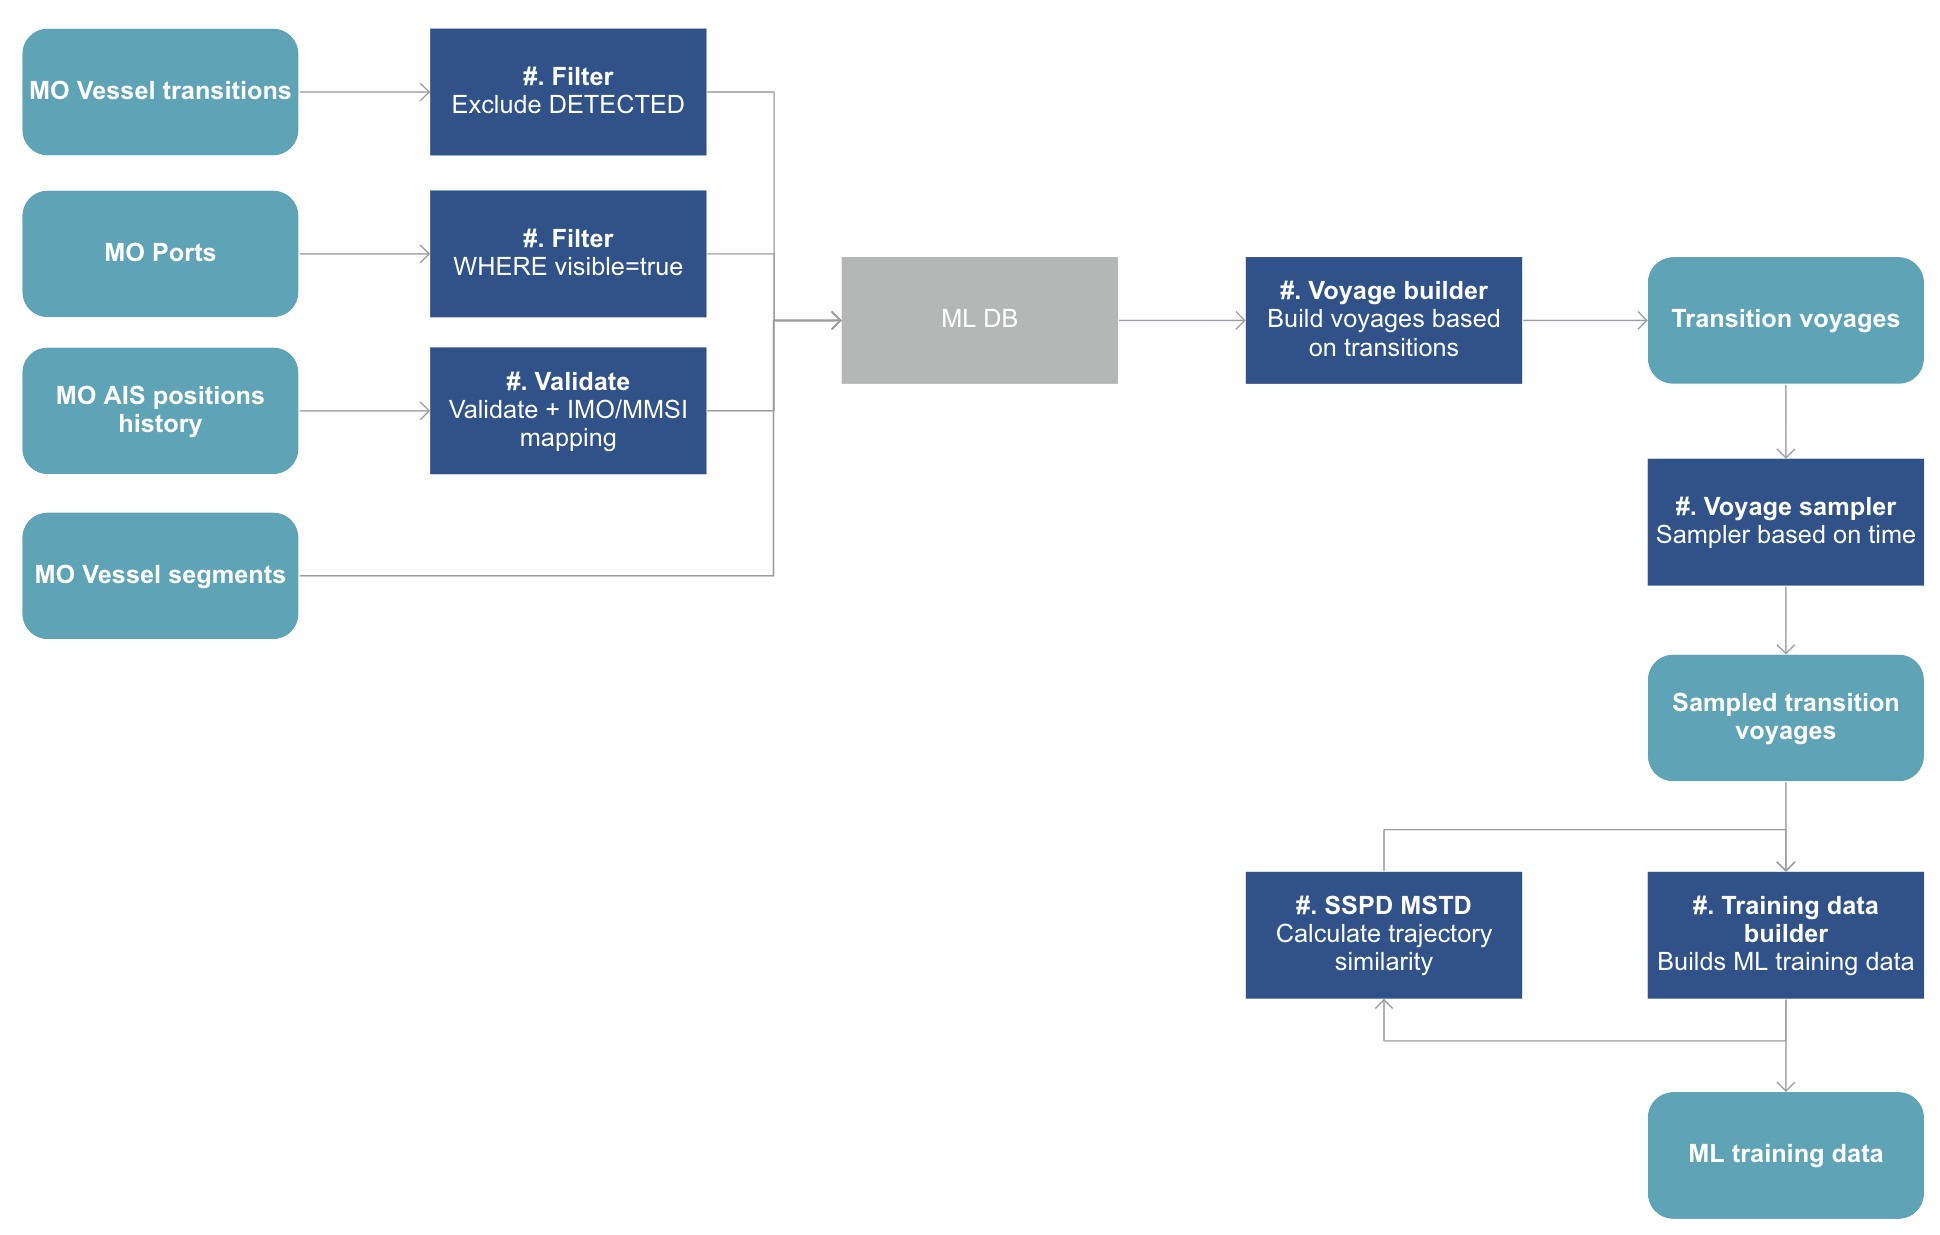
\includegraphics[width=1.0\textwidth]{figures/dataset_overview}
    \caption{Overview of the process used to construct the dataset used in further analysis and \acrshort{ml}.}
    \label{fig:dataset_overview}
\end{figure}

\begin{table}[htbp]
    \centering
    \small{\begin{tabularx}{1.0\textwidth}{p{1.0in} p{0.75in} X}
        \bfseries{Column} & \bfseries{Type} & \bfseries{Description} \\ \toprule
        id & serial int & unique identifier \\ \midrule
        voyage\_id & int & the original voyage id from sampled transition voyages \\ \midrule
        imo & int & identifier for the traveling vessel\\ \midrule
        mmsi & int & identifier for the traveling vessel\\ \midrule
        segment & string & the vessel's segment \\ \midrule
        sub\_segment & string & the vessel's sub-segment \\ \midrule
        departure\_port & string & \gls{locode} of the vessel's departure port \\ \midrule
        trajectory\_length & int & number of points in the sampled trajectory \\ \midrule
        sspd\_mstd & string & \gls{locode} of the \acrshort{mstd} value for the voyage trajectory \\ \midrule
        sspd\_dist & int & similarity value between the voyage trajectory and the most similar historical trajectory   \\ \midrule
        arrival\_port & string & \gls{locode} of the vessel's arrival port \\ \bottomrule
    \end{tabularx}}
\caption{Final structure of the ml\_training\_data database table.}\label{tab:ml_training_data}
\end{table}

\section{ML-based training and destination prediction}

After building the \acrfull{ml} training dataset, the next part of the process included finding a \acrshort{ml} model that suits the dataset, prepare and train it to predict values for the arrival port column in the training dataset. This section describes the process starting from the training dataset to the final trained prediction model.

\subsection{Categorical label encoding}

In the training dataset, there are both numerical values as well as categorical values. Categorical values are values that are a subset of a finite number of possible values, while numerical values have infinite possible values. In the training data, the data concerning ports and vessel segments are examples of categorical values, and the length of the vessel trajectories and the similarity values derived from the \acrshort{mstd} value is numerical. As described in \cref{sec:label_encoding}, the categorical values must be encoded so that \acrshort{ml} models can understand them. Choosing an appropriate encoding method depends on the cardinality of the features in the dataset. For instance, there are more than 5000 possible ports in the data foundation, therefore, columns concerning ports such as arrival port, departure port, and \acrshort{mstd} have high cardinality. On the other hand, the features segment, and sub-segment have lower cardinality as there are only eight segments and 95 unique sub-segments. Based on the advantages and disadvantages of label encoding and ``one-hot'' encoding (\cref{sec:label_encoding}), it makes sense to ``one-hot'' encode the low cardinality features, while using label encoding for the remaining columns.

\todo{figure or code}

\subsection{Dataset imbalance}
\label{sec:dataset_imbalance}

Due to the nature of vessel voyage patterns based on vessels of different types and sizes, there is a substantial imbalance in the number of voyages arriving at different ports. In other words, there is a severe imbalance in occurrences of arrival port values in the training set. \cref{fig:data_imbalance} shows the distribution of frequencies of voyages arriving at different ports, and as it shows, there is a significant imbalance in this distribution.

\begin{figure}[htbp]
    \centering
    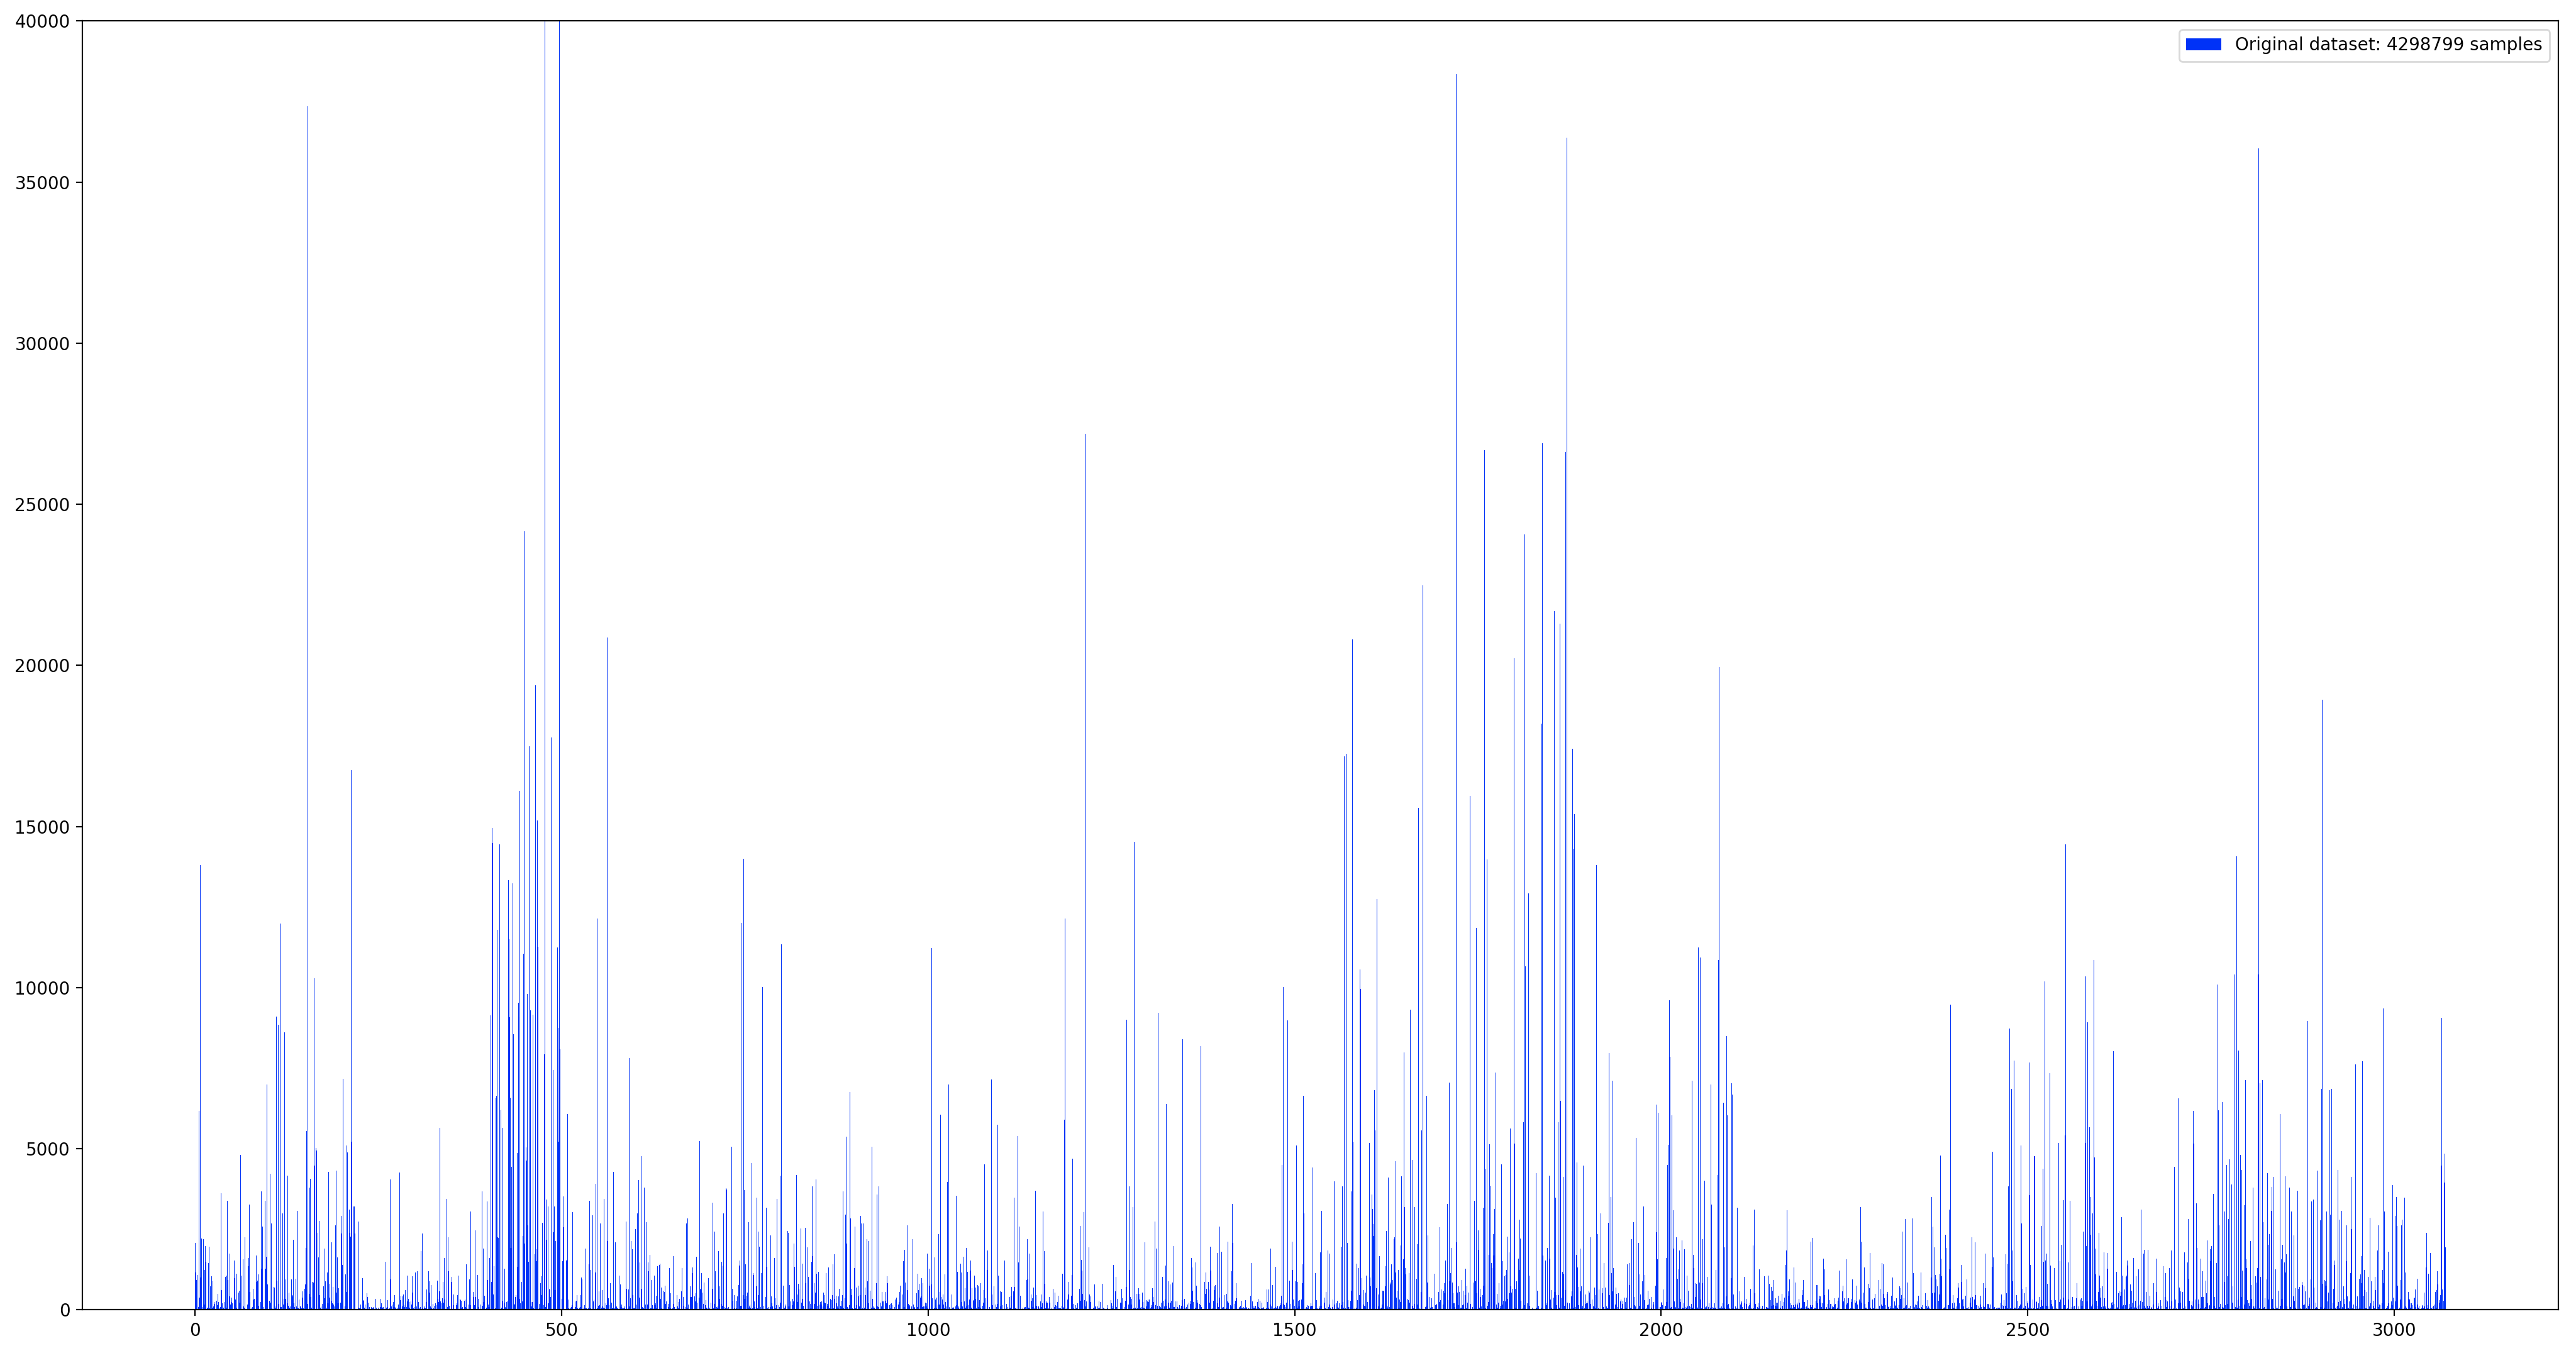
\includegraphics[width=0.8\textwidth]{figures/imbalance/original}
    \caption{Graph showing the distribution of frequencies among the arrival port classes.}
    \label{fig:data_imbalance}
\end{figure}

Because of the severe imbalance in the training set, simply applying oversampling techniques on the full dataset such as \acrshort{smote} to the original dataset increases the total data size to an unmanageable amount of \textbf{203} million samples. On the other hand, using a simple majority undersampling method removes most of the data, reducing it so almost no data is left. \cref{fig:all_samplers} shows how different sampling methods perform using a limited version of the original dataset. As it shows, \acrshort{smote} (purple graph), oversamples the dataset massively, undersampling (red graph) reduces the dataset by \textit{92\%}, while \acrshort{smote} + ENN increases data size, but does a better job keeping relationships in the data.

\begin{figure}[htbp]
    \centering
    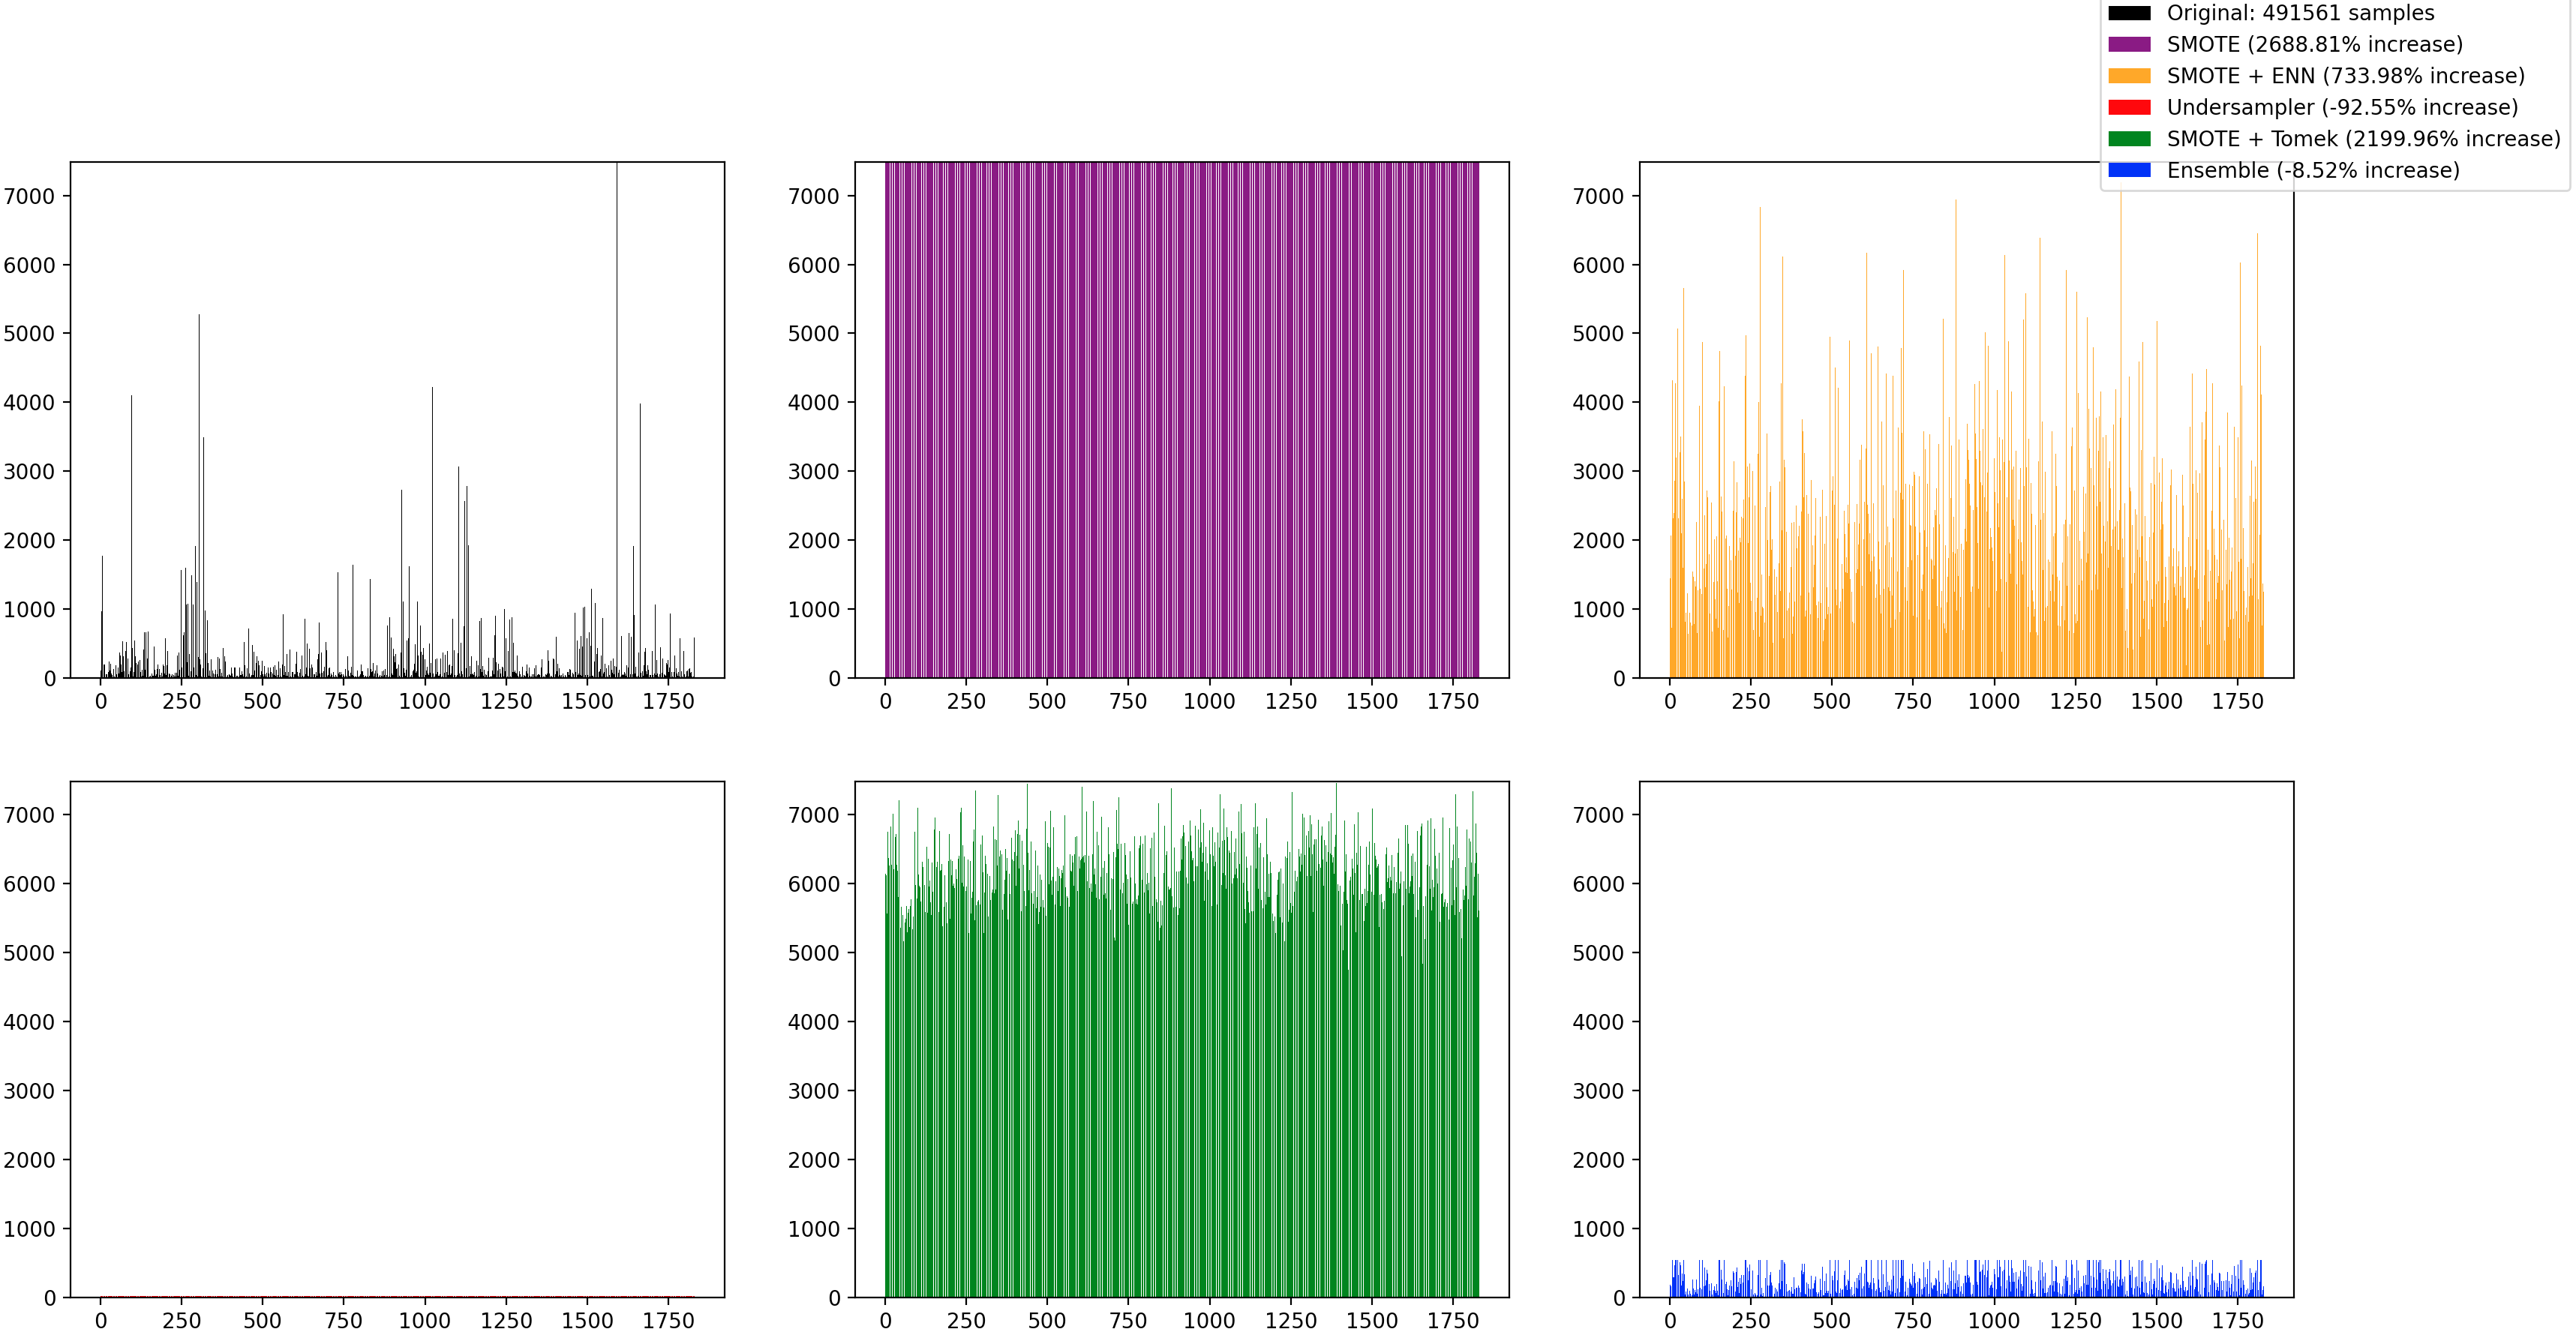
\includegraphics[width=1.0\textwidth]{figures/imbalance/all_samplers}
    \caption{Different sampling methods compared based on the increase in data size.}
    \label{fig:all_samplers}
\end{figure}

Because of the significant outliers in the data, an ensemble of both under and oversampling was used to balance the dataset without generating a massive amount of synthetic data while also not removing too much information. The ensemble approach first undersamples classes that occur more than \textit{20\%} of the most frequent class to remove the most severe spikes, applies \textit{``\acrshort{smote} + ENN''} over and undersampling method to balance the dataset while still keeping important patterns in the dataset, then finally an undersampling step is added to flatten out frequency spikes to arrive at a final dataset size that is similar to the original. However, since \acrshort{smote} is used during this process, there are synthetic samples in the new dataset. These generated values are based on similar samples in the dataset, however, in the case of segment and sub-segment, specific sub-segments belong to certain segments, so when these are structured as separate values, SMOTE can synthetically generate invalid combinations of segments and sub-segments. To ensure the model doesn't waste time training on impossible segment and sub-segment combinations, the segment and sub-segment values were combined into one segmentation value before encoding and balancing. This also reduces the complexity of the \acrshort{ml} model structure as there are one fewer feature to consider. The segment and sub-segment values are concatenated using a delimiter, so they are easily divided again after training to further evaluate the results based on these values.

\subsection{Model selection}

At this stage, the final data is fully processed and prepared for model training. However, first, the model that best fits the dataset must be chosen. In this process, several different classifiers were tested out with a smaller extract of the training data. Using Python libraries such as ``Scikit-Learn'' and XGBoost, the \acrshort{ml} models tested are listed in \cref{tab:model_selection}.

\begin{table}[htbp]
    \centering
    \small{\begin{tabularx}{1.0\textwidth}{p{1.0in} X p{0.7in}}
            \bfseries{Model} & \bfseries{Description} & \bfseries{Acc. \%} \\ \toprule
            Random Forest & Ensemble tree-based algorithm where trees are built using a random number of features. & 91.6 \\ \midrule
            XGBoost & Extreme gradient boosting. Ensemble tree-based algorithm where trees are constructed building on mistakes from previous trees.. & 89.9 \\ \midrule
            One vs. Rest XGBoost & Train a binary XGBoost classifier for every possible arrival port.  & 89.5 \\ \midrule
            k-Nearest Neighboor & kNN - samples look at their n neighbors to classify themselves. & 77.4 \\ \midrule
            Tensorflow + keras DNN & Deep neural network for multiclass classification. Nodes in sequential hidden layers are fitted based on an activation function. & 50 \\ \midrule
            One vs. Rest Multi-layered perceptron & Deep neural network -based binary classifier for every possible arrival port. & 10 \\ \bottomrule
    \end{tabularx}}
\caption{Classifiers tested out in the model selection phase. Every classifier was trained using 50 thousand samples from the training data.}\label{tab:model_selection}
\end{table}

\todo{perhaps I should move more explanation over to background}

Note that One vs. Rest (OVR) classifiers differs from the multi-class classification methods as they convert the multi-class problem to multiple binary classification problems. For instance, instead of predicting which port a voyage will arrive at, the OVR classifiers consider the perspective of a port so that the problem becomes: will the vessel arrive at this specific port? Moreover, the best performing model was the \acrfull{rf} model, followed closely by the two variants of XGBoost implementations. The \acrshort{rf} and \acrshort{xgb} models are somewhat similar methods. They both are both ensemble decision tree methods meaning they configure multiple decision trees, or a forest, that vote on outcome values. This is based on the concept of ``wisdom of crowds'' where multiple relatively uncorrelated trees acting as a committee is capable of outperforming a single decision tree classifier. In the \acrshort{rf} method, the decision trees are constructed using bagging and bootstrapping as methods of randomizing the construction of decision trees either by randomizing what features to use when constructing a tree or what samples to use. The goal is that the trees gain their own unique perspective by being constructed in a particular way. In the \acrshort{xgb} model, trees are created in a process called boosting where in each boosting round a new tree is constructed based on the previous mistakes made by the previous trees.

Initially, the \acrshort{rf} model was explored further for the final training process. However, the ``RFClassifier'' Python implementation seemed problematic for larger datasets as the memory requirements are considerable because of the size of the model as well as the high number of possible arrival ports which requires a large tree ensemble to learn. Furthermore, the Python implementation does not support out-of-core learning or incremental batch learning so it is less practical in the final training process. On the other hand, the XGBoost implementation seems more apt at handling larger data sizes as it uses less memory in general as well as it supports both out-of-core and incremental learning which is provides more options in terms of computing resource requirements.

\subsection{Configuration and parameter optimization}

For different \acrshort{ml} methods, there are usually many different configurations available to tune how the model learns. For the selected \acrfull{xgb} model, based on the library's documentation, the most important parameters to configure are the following:

\begin{itemize}
    \item \textit{n\_estimators} - the number of boosting rounds used. Default is 100.
    \item \textit{max\_depth} - the max depth per tree in the model. Default is 6.
    \item \textit{subsample} - the fraction of samples from the training data considered when building each tree. Default is 1.0.
    \item \textit{colsample\_bytree} - the number of features to consider when building each tree. Default is 1.0.
    \item \textit{min\_child\_weight} - the minimum weight required for a child node. Default is 1.0.
    \item \textit{gamma} - the minimum loss reduction required to split a node in the tree. Default is 0.
\end{itemize}

The parameters \textit{n\_estimators}, \textit{max\_depth}, \textit{min\_child\_weight}, and \textit{gamma} helps control the complexity of the model, while the others introduce randomness to the tree building process. All of these parameters can be tuned to prevent overfitting and produce a well-performing model. In order to find the best parameters to use, the model was trained several times using different configurations on a subset of the original dataset in a process called hyper-parameter optimization. First, the parameters listed above were listed with a range of different values for each to test. Initially, these ranges were large to get an initial idea of what parameters fit the best. A random grid search was used to find a rough estimate of what values perform the best. In this process, 100 different configurations were randomly selected from all the possible permutations in order to get a feeling of what types of ranges fit the different parameters without attempting to train on all of them. The best result from this process provided insight into what general values seemed to work for the dataset. \cref{lst:grid_search} shows an example of how parameters are defined and used in a random search. Next, a grid search was applied using smaller ranges based on the best result from the random search to further fine-tune the parameters. The grid search methods both use cross folder validation to arrive at the best performing configuration to consider overfitting in the final result, so the resulting parameters are a good place to start in the initial training process.

\begin{lstlisting}[
    caption={Python example of parameters used for random grid search in hyper-parameter optimization process.},
    label=lst:grid_search,
    language=Python,
    showstringspaces=false,
]
random_grid = {
    "n_estimators": [100, 200, 300],
    "max_depth": [6, 8, 10],
    "subsample": [0.6, 0.8, 1.0],
    "learning_rate": [0.1, 0.2, 0.3],
    "colsample_bytree": [0.7, 0.8, 0.9, 1.0],
    "min_child_weight": [1, 2, 5, 8],
    "gamma": [0.0, 0.1, 0.2, 0.3],
}

# ...

best_params = best_random.random_search_cv(X_train, y_train, random_grid)
print("Best params from random search")
pprint(best_params)

# ...

def random_search_cv(self, X, y, param_grid, folds=3):
    # Random search of parameters, using X-fold cross validation,
    # search across 100 different combinations, and use all available cores
    self.classifier = RandomizedSearchCV(estimator=self.classifier,
                                         param_distributions=param_grid,
                                         n_iter=100, cv=folds, verbose=3,
                                         random_state=42, n_jobs=-1)

    # Fit the random search model
    self.classifier.fit(X, y)
    return self.classifier.best_params_

\end{lstlisting}


\subsection{The training process}
\label{sec:training_process}

After finding appropriate parameters for the model, the next step was to conduct the training process. The process is straightforward, however, the size of the training set resulted in high computing requirements, especially in terms of available RAM on the running computer. \acrshort{xgb} supports both iterative and external memory training routines, therefore, these alternatives were also evaluated to see what method works best. In total, the three alternatives available for the training process were: training the model iteratively by dividing the training data into multiple batches, using the computer's hard drive as memory using \acrshort{xgb}'s external memory mode, or simply training the model normally using a computer with sufficient hardware requirements. The training process was conducted using the full dataset containing \textbf{4.3} million voyages which were encoded and balanced beforehand. The training set was divided into \textit{80\%} training data and \textit{20\%} testing data which was used to estimate the performance of the model.

Moreover, the aforementioned approaches were initially tested using a computer with an \textit{AMD Ryzen 7 2700} processor with 8 physical CPU cores and 8 additional virtual ones, an \textit{NVIDIA GeForce GTX 1080} GPU, and 48GB of available RAM\@.

First, the full training set was used in the standard training process. However, this process demanded more memory than available on the machine. By trial and error, it was established that 48GB of memory was only sufficient to train on a subset of around 1 000 000 samples. Thus, the iterative training approach was tested using a limited subset of the available data in different batches. In this process, the full dataset was fetched, encoded, and balanced before it was split into batches. As the entire dataset was kept in memory during the batch process, the batch size was set to 600 000 for the iterative training process. For this process, the additional parameters \textit{updater} and \textit{process\_type} were set to ``refresh'' and ``update'' respectively in order to ensure that the model correctly adapts to exposure to new samples. \cref{lst:batch_train} shows the code used to prepare data into batches and iteratively train the model.

\begin{lstlisting}[
    caption={Python functions used to batch train the XGBoost model.},
    label=lst:batch_train,
    language=Python,
    showstringspaces=false,
]
def prepare_training_data(config):
    df = get_all_data()
    df = df.groupby(config["t_column"]).filter(lambda x: len(x) >= 20)

    X, y = encode(df, config)

    if config["sample"] == True:
        X, y = ensemble_sampler(X, y)
        inc = (len(X)-len(df))/len(df)*100
        print("[main] sampled data: {:.2f}% increase".format(inc))

    X_train, X_test, y_train, y_test = train_test_split(
        X, y, test_size=0.20, random_state=42)
    batches = []
    for x in batch(range(0, len(X_train)), config["batch_size"]):
        batches.append(x)

    return batches, X_train, X_test, y_train, y_test

def batch_train_model(batches, X_train, X_test, y_train, y_test):
    params = {
        # ... other params
        "updater": "refresh",
        "process_type": "update",
        "num_class": len(np.unique(pd.concat([y_train, y_test]))),
    }

    # XGBoostClassifier is a custom wrapper around the XGBClassifier class.
    classifier = XGBoostClassifier(target_column="arrival_port", params=params)
    trained_model = None
    for t_indices in batches:
        # subset training data
        X = X_train.iloc[t_indices]
        y = y_train.iloc[t_indices]

        # eval set using the total training data
        dtrain = xgb.DMatrix(data=X_train, label=y_train)
        dtest = xgb.DMatrix(data=X_test, label=y_test)
        watchlist = [(dtest, 'eval'), (dtrain, 'train')]

        # train the model
        trained_model = classifier.train_model(
            X, y, model=trained_model, num_boost_round=100, watchlist=watchlist)
        classifier.print_evaluate_summary(X_test, y_test, matrix=True)

    return classifier, X_train, X_test, y_train, y_test
\end{lstlisting}


Next, the external memory version of \acrshort{xgb} was tested in an attempt to run the training process in one training round using the machine's hard drive as additional memory. In this process, the full dataset was fetched, sampled, and balanced before it was written to a \textit{libsvm} file as recommended by the library's documentation. The algorithm then produces a memory-optimized cache file on the computer's disc which is then used in the training process. \cref{lst:ext_mem_train} shows how \acrshort{xgb}'s ``train'' API can be modified to use external memory where the file name specifies ``train.txt'' as the input file using ``dtrain.cache'' as a temporary cache file.

\begin{lstlisting}[
    caption={Python code showing how a \acrshort{xgb} model can be trained using external memory.},
    label=lst:ext_mem_train,
    language=Python,
    showstringspaces=false,
]
# internal memory version
# dtrain = xgb.DMatrix(data=X, label=y)

# external memory version
train_file = "train.txt#dtrain.cache"
dtrain = xgb.DMatrix("{:s}/{:s}".format(data_folder, train_file))

clf = xgb.train(self.params,
                dtrain,
                #... other parameters
            )
\end{lstlisting}

Finally, in order to establish the differences and to find the most optimal training process, a standard training process was tested on the full dataset on a more powerful computer. In this process, a virtual machine hosted on the collaborative company \acrfull{mo}'s cloud computing environment was used in the training process. This machine has 256GB of available memory and 32 virtual CPU cores. This was sufficient to train the full dataset and was the preferred method as it also allowed testing other \acrshort{ml} models that do not support incremental or external memory training processes. \cref{lst:final_training_process} shows the code used to train the final model. An evaluation set was provided to the model to continuously evaluate it after each decision tree has been built in the model. It also allows for plotting performance metrics over each ``boosting round'' which can be helpful to detect when in the training process the model can become overfitted.

\begin{lstlisting}[
    caption={Python code showing how the \acrshort{xgb} model was trained in one iteration},
    label=lst:final_training_process,
    language=Python,
    showstringspaces=false,
]
def train_xgb_classifier(df, target_column):
    params = {
        "use_label_encoder": False,
        "objective": "multi:softmax",
        "learning_rate": 0.1,
        "n_estimators": 100,
        "max_depth": 4,
        "subsample": 0.8,
        "gamma": 0.2,
        "eta": 0.2,
    }

    classifier = XGBoostClassifier(target_column=target_column, params=params)

    X_train, X_test, y_train, y_test = classifier.train_test_split(df, balance=True)

    # eval_set allows continuous evaluation during the training process
    eval_set = [(X_train, y_train), (X_test, y_test)]

    # fit the model (esr = early_stopping_rounds)
    classifier.fit_model(X_train, y_train, eval_set=eval_set,
                        esr=5, plot_results=True)

    return classifier, X_train, X_test, y_train, y_test
\end{lstlisting}

The results from the training processes are later discussed in \cref{chap:results}.

\subsubsection{Evaluation process}
\label{sec:evaluation_process}

For all of the different training processes tested, the same evaluation process was used in order to establish the performance of the model. First, to detect if the trained model is overfitted, three-fold cross-validation applied during the training process. In this process, the model is trained three times using different parts of the training set as training and evaluation data. If the performance of each training process does not deviate significantly, the model is less likely to be overfitted and should be able to efficiently predict previously unseen samples. Moreover, plotting performance metrics for each iteration of the training process also provides insight into when the model stops learning and starts to overfit.

Based on \acrshort{ml} conventions and related works, several performance metrics were used in addition to conventional accuracy. As already mentioned in \cref{sec:dataset_imbalance}, accuracy can be a misleading metric in some cases such as for imbalanced datasets. This is, however, a smaller issue after sampling has been used to balanced the dataset beforehand, but other performance metrics still provide more insight into the performance of the model. In addition to accuracy, the metrics, \textit{logarithmic loss}, \textit{classification error}, \textit{precision}, \textit{recall}, and \textit{F1 score} were used. Furthermore, to gain more insight into the model performance on the particular dataset, accuracies per segment and sub-segment were also collected as listed in \cref{lst:segment_accuracy}. Furthermore, this helps to gain insight into the traveling patterns of different vessel types as it pertains to the predictability of vessels of different types and sizes.

\begin{lstlisting}[
    caption={Python code used to calculate accuracies per segment and sub-segment to gain insight into the predictability of different vessels.},
    label=lst:segment_accuracy,
    language=Python,
    showstringspaces=false,
]
def column_accuracy(correct, incorrect, columns=["segment", "sub_segment"]):
    cr = correct.groupby(columns).size()
    cr.name = "correct"
    icr = incorrect.groupby(columns).size()
    icr.name = "incorrect"

    df = pd.concat([cr, icr], axis=1).fillna(0)
    df["total"] = df["correct"] + df["incorrect"]
    df = df.astype({ "correct": "int32", "incorrect": "int32", "total": "int32" })
    df["accuracy"] = df["correct"]/df["total"]

    # sort groups by accuracy if grouped by more than 1 column
    if len(columns) > 1:
        g = df["accuracy"].groupby(columns[0], group_keys=False)
        res = g.apply(lambda x: x.sort_values(ascending=False))
        return res

    return df.sort_values(by=["accuracy"], ascending=False)
\end{lstlisting}

\section{Vessel destination prediction method summary}

After the training process, the final trained model is saved and can then be used to predict the outcome of new samples of traveling voyages. To predict a traveling vessel's next destination, the steps described throughout this chapter must be replicated for that single vessel. Given the trained model, the overall prediction process for a single traveling vessel can be conceptualized using the following steps:

\begin{itemize}
    \item The current trajectory of the traveling vessel is collected using \acrshort{ais} records ranging from the last transmitted \textit{``MOORED''} status to its current position along with the id (\gls{locode}) of the departure port where it was moored and the vessel's segmentation values.
    \item The vessel's trajectory is then sampled based on a predefined time interval, then compared to every historical outgoing trajectory from the same departure port from vessels of the same segment and sub-segment to establish the \acrfull{mstd}.
    \item The vessel's segment, sub-segment, departure port, trajectory length, \acrshort{mstd}, and the \acrshort{mstd} similarity value is then passed to the trained \acrshort{xgb} model that predicts the traveling vessel's arrival port.
\end{itemize}
